\documentclass[warsaw, 9pt]{beamer}
\usepackage[T1]{fontenc}
\usepackage[utf8]{inputenc}
\usepackage{lmodern}

\usepackage{amsfonts,amsmath}
\allowdisplaybreaks


%% X color
\definecolor{darkblueX}{RGB}{0,62,92}
\definecolor{lightblueX}{RGB}{0,104,128}
\definecolor{verylightblueX}{RGB}{212,232,239}
\definecolor{redX}{RGB}{169,32,33}

%% Set new default colors
\setbeamercolor{title}{fg=white, bg=darkblueX}
\setbeamercolor{frametitle}{fg=darkblueX, bg=white}
\setbeamercolor{block body}{bg=verylightblueX}%
\setbeamercolor{block title}{bg=darkblueX,fg=white}%
\setbeamercolor{structure}{fg=darkblueX,bg=white}
\setbeamercolor{normal text}{fg=darkblueX,bg=white}%

\setbeamercolor{alerted text}{fg=redX}


%% Font

\setbeamerfont{framesubtitle}{size=\tiny}
\setbeamerfont{alerted text}{shape=\bfseries}




%\usepackage[export]{adjustbox}

% Tighter itemize
\expandafter\def\expandafter\normalsize\expandafter{%
    \normalsize%
    \setlength\abovedisplayskip{1pt}%
    \setlength\belowdisplayskip{1pt}%
    \setlength\abovedisplayshortskip{1pt}%
    \setlength\belowdisplayshortskip{1pt}%
}

\expandafter\def\expandafter\small\expandafter{%
    \small%
    \setlength\abovedisplayskip{1pt}%
    \setlength\belowdisplayskip{1pt}%
    \setlength\abovedisplayshortskip{1pt}%
    \setlength\belowdisplayshortskip{1pt}%
}

%\usepackage{beamerX}
\newcommand{\alertmath}[1]{\textcolor{redX}{\boldsymbol{#1}}}
%\setboolean{displaylogo}{false}

\AtBeginSection[]
{
\begin{frame}
        \frametitle{Outline}
        \tableofcontents[currentsection]
   \end{frame}
}
\AtBeginSubsection[]
{
\begin{frame}
        \frametitle{Outline}
        \tableofcontents[currentsection,currentsubsection]
   \end{frame}
}

\setbeamertemplate{frametitle continuation}[from second][]

\usepackage{graphicx}%
\graphicspath{{./}{./Figures/}}
\newcommand{\parinc}[2]{\parbox[c]{#1}{\includegraphics[width=#1]{#2}}}
\newcommand{\parinch}[3]{\parbox[c][#2]{#1}{\includegraphics[width=#1]{#3}}}
\newcommand{\parincb}[3]{\parbox[c]{#1}{\includegraphics[width=#1,height=#2]{#3}}}

\usepackage{color}
\newcommand{\red}[1]{\textcolor{red}{#1}}

\usepackage{tikz}


\usepackage{scalerel,stackengine}
\stackMath
\newcommand\reallywidehat[1]{%
\savestack{\tmpbox}{\stretchto{%
  \scaleto{%
    \scalerel*[\widthof{\ensuremath{#1}}]{\kern-.6pt\bigwedge\kern-.6pt}%
    {\rule[-\textheight/2]{1ex}{\textheight}}%WIDTH-LIMITED BIG WEDGE
  }{\textheight}% 
}{0.5ex}}%
\stackon[1pt]{#1}{\tmpbox}%
}

\newcommand{\grad}{\nabla}
\newcommand{\ind}[1]{\mathbf{1}_{#1}}

\DeclareMathOperator{\limSup}{limsup}%
\DeclareMathOperator{\limInf}{liminf}%
\DeclareMathOperator*{\argmax}{argmax}%
\DeclareMathOperator*{\argmin}{argmin}%
\DeclareMathOperator*{\supp}{Supp}%
\DeclareMathOperator{\pen}{pen}
\DeclareMathOperator{\dom}{dom}
\DeclareMathOperator{\price}{price}
\DeclareMathOperator{\sign}{sign}
\DeclareMathOperator{\KL}{KL}
\DeclareMathOperator{\Proj}{Proj}
\DeclareMathOperator{\Span}{span}


\DeclareMathOperator*{\tr}{tr}
\DeclareMathOperator*{\ra}{rank}
\DeclareMathOperator*{\conv}{conv}
\DeclareMathOperator{\ve}{vec}
\DeclareMathOperator{\diag}{diag}


\newcommand{\Proba}{\mathbb{P}}
\newcommand{\Espe}{\mathbb{E}}
\newcommand{\Vari}{\mathbb{V}}
\newcommand{\Cova}{\mathbb{C}\text{ov}}
\newcommand{\Prob}[2][]{\Proba_{#1}\left\{#2\right\}}
\newcommand{\Esp}[2][]{\Espe_{#1}\left[#2\right]}
\newcommand{\Var}[2][]{\Vari_{#1}\left[#2\right]}
\newcommand{\Cov}[2][]{\Cova_{#1}\left[#2\right]}
\newcommand{\ud}{\textup{d}}
\newcommand{\charac}{\mathbf{1}}

\newcommand{\vecX}{\textbf{X}}
\newcommand{\vecx}{\textbf{x}}
\newcommand{\transp}[1]{{#1}^t}
\usetheme{Boadilla}
\usepackage{pdfpages}
\usepackage{tikz}
\usepackage{dsfont}

\usepackage[style=alphabetic, citestyle = authoryear, maxcitenames=2,backend=biber]{biblatex}
\addbibresource{../deeplearning_course.bib}
%Compile pdflatex, biber, pdflatex, pdflatex

\newcommand\citem[1]{{\scriptsize[\citetitle{#1}, \cite{#1}]}}

\newcommand\redd[1]{\textcolor{red}{#1}}
\newcommand\blue[1]{\textcolor{blue}{#1}}
\newcommand\iid{\textit{i.i.d.}}
\newcommand\R{\mathds{R}}
\newcommand\bx{\mathbf{x}}
\renewcommand\pen{\textrm{pen}}
\newcommand{\E}{\mathds{E}}
\newcommand{\V}{\mathds{V}}
\newcommand{\cov}{\mathds{C}}
\renewcommand{\P}{\mathds{P}}

\usepackage{ifthen}
\newboolean{correction_bool}
\setboolean{correction_bool}{false}
\newcommand{\ifinclude}[1]{\ifthenelse{\boolean{correction_bool}}{#1}{}}

\usepackage{graphicx}
\graphicspath{{../}}
\usepackage{ragged2e}




\title[Deep Learning]{Convolutional Neural Networks\\
\small
}

\author{E. Scornet}

\date{Fall 2018}

\begin{document}

\begin{frame}
  \titlepage
\end{frame}




\begin{frame}
	\frametitle{Neural Network reborn}
	


\blue{Renewed interest in 2006}: 
\citem{hinton2006fast}

\smallskip

Propose a way to train deep neural nets: 
\begin{itemize}
	\item Train the first layer. 
	\item Add a layer on top of it and train only this layer. 
	\item Repeat the process until the network is deep enough.
	\item Use this network as a warm start to train the whole network.
\end{itemize}

\bigskip

\blue{Technical reasons} for this new growing interest: 
\begin{itemize}
	\item Larger datasets
	\item More powerful computers
	\item Software infrastructure
	\item Small number of algorithmic changes
	\begin{enumerate}
		\item MSE replaced by cross-entropy
		\item ReLU (Fukushima, 1975, 1980)
	\end{enumerate}
\end{itemize}
\end{frame}








\begin{frame}
	\frametitle{Using classical networks for images?}
	
\blue{No}, for two reasons: 
	\begin{itemize}
		\item Non robust to image shifting 
		\item Do not take into account the spatial organization of pixels (if the pixels are permuted, the output of the network would be the same, whereas the image would change drastically).
	\end{itemize}

\medskip

\blue{Idea}: 
\begin{itemize}
	\item Apply local transformation to a set of nearby pixels (spatial nature of image is used)
	\item Repeat this transformation over the whole image (resulting in a shift-invariant output).
\end{itemize} 

\medskip

\blue{Not a new idea}: trace back to perceptron and study about the visual cortex of a cat. 

The cat is able to
\begin{itemize}
	\item detect oriented edges, end-points, corners (low-level features)
	\item combine them to detect more complex geometrical forms (high-level features)
\end{itemize} 



\end{frame}


\section{Foundations of CNN}



%
%\begin{frame}
%	\frametitle{}
%	
%	\small
%	
%	We will go into more details below, but a simple ConvNet for CIFAR-10 classification could have the architecture [INPUT - CONV - RELU - POOL - FC]. In more detail:
%	
%	\begin{itemize}
%		\item INPUT [32x32x3] will hold the raw pixel values of the image, in this case an image of width 32, height 32, and with three color channels R,G,B.
%		
%		\item 	CONV layer will compute the output of neurons that are connected to local regions in the input, each computing a dot product between their weights and a small region they are connected to in the input volume. This may result in volume such as [32x32x12] if we decided to use 12 filters.
%		
%		\item 	RELU layer will apply an elementwise activation function, such as the $\max(0,x)$ thresholding at zero. This leaves the size of the volume unchanged ([32x32x12]).
%		
%		\item 	POOL layer will perform a downsampling operation along the spatial dimensions (width, height), resulting in volume such as [16x16x12].
%		
%		\item 	FC (i.e. fully-connected) layer will compute the class scores, resulting in volume of size [1x1x10], where each of the 10 numbers correspond to a class score, such as among the 10 categories of CIFAR-10. As with ordinary Neural Networks and as the name implies, each neuron in this layer will be connected to all the numbers in the previous volume.
%	\end{itemize}
%	
%
%\end{frame}



\subsection{Convolution layer}

\begin{frame}{Convolutional neural networks (CNNs)}
	\begin{itemize}
		\item Neural networks that use \textbf{convolution instead of matrix product} in one of the layers
		
		\medskip 
		
		\item A CNN layer typically includes 3 operations: \textbf{convolution}, \textbf{activation} and \textbf{pooling}
		
		\medskip 
				
		\item Using the more general idea of \textbf{parameters sharing}, instead of \textbf{full connection} (convolution instead of matrix product)
	\end{itemize}
	
	\bigskip 
	
	Convolution operator in neural networks is as follows
	
	\begin{equation*}
		O(i, j) = (I \star K)(i, j) = \sum_{k} \sum_{l} I(i + k, j + l) K(k, l)
	\end{equation*}
	\begin{itemize}
		\item $I$ is the input and $K$ is called the kernels
		\item The kernel $K$ will be \textbf{learned} (replaces the weights $\mathbf{W}$ in a fully connected layer)
	\end{itemize}
\end{frame}

\begin{frame}
	\frametitle{Convolution - Grey scale}

\begin{itemize}
	\item Size of the input image is $8 \times 8 \times 1$ (height, width, depth)
	
	\medskip 
	
	\item Size of the kernel is $3 \times 3 \times 1$
\end{itemize}

\begin{center}
	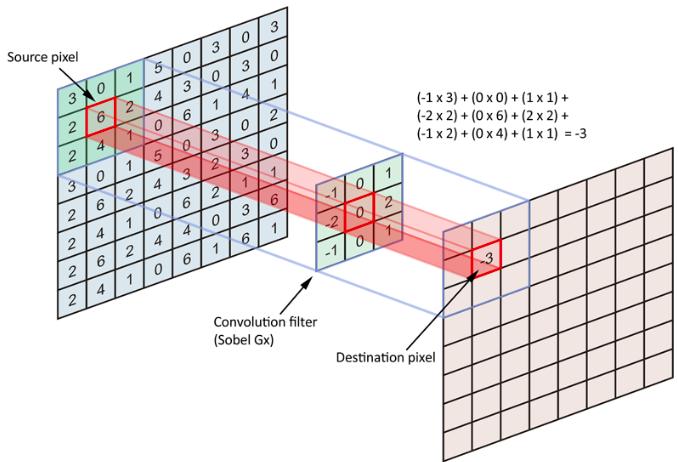
\includegraphics[scale=0.3]{figs/convolution.png}
\end{center}
	
\end{frame}












\begin{frame}
	\frametitle{Convolution - RGB}
	
\begin{itemize}
	\item Size of the input image is $8 \times 8 \times 3$ (height, width, depth)
	\item Size of the kernel is $3 \times 3 \times 3$
\end{itemize}

	\begin{center}
		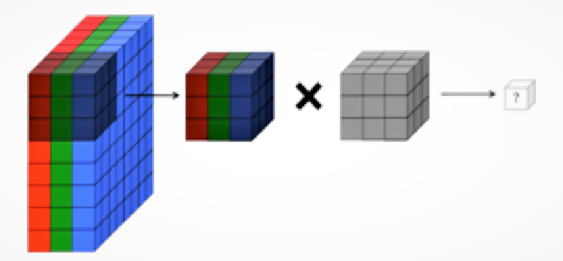
\includegraphics[scale=0.9]{figs/kernel_volume.png}
	\end{center}

Warning: every filter is small spatially (along width and height), but extends through the full depth of the input volume.


\end{frame}


\begin{frame}
	\frametitle{Parameters for convolutional layer 1/3}
	
	Three hyperparameters control the size of the output volume: the depth, stride and zero-padding.
	
	\begin{itemize}
		\item The \blue{depth of the output volume}, i.e., the number of filters/activation maps/feature maps.
	\end{itemize}
	
	
	

		\begin{center}
			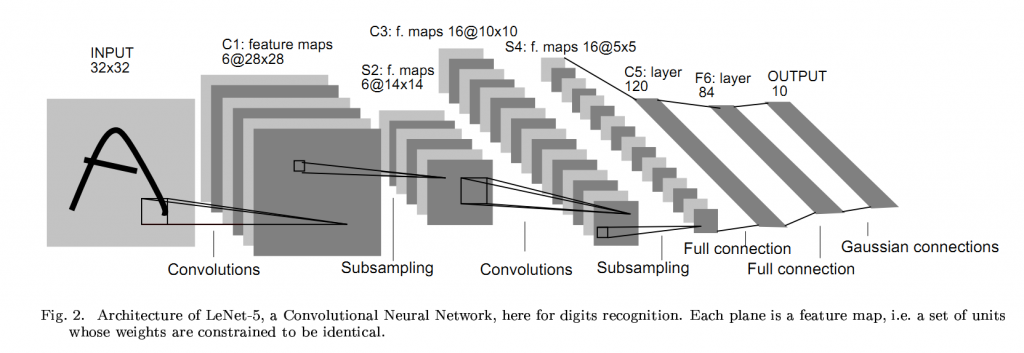
\includegraphics[scale=0.3]{figs/LeNet}
		\end{center}
	
	
\end{frame}

\begin{frame}
	\frametitle{Parameters for convolutional layer 2/3}
	
	Three hyperparameters control the size of the output volume: the depth, stride and zero-padding.
	
	\bigskip 
	
	\begin{itemize}
		\item The \blue{depth of the output volume},
		
		\item The \blue{stride}, i.e., of how many pixels do we move the filter horizontally and vertically. Usually, stride is equal to one (rarely to two, and even more rarely larger).
	\end{itemize}

	
	\begin{columns}[T] % align columns
		\hspace{0.2cm}
		\begin{column}{.5\textwidth}
			Stride $=1$
			\begin{center}
				\includegraphics[scale=0.4]{figs/stride1}
			\end{center}
		\end{column}%
		\vrule{}
		\hspace{0.2cm}
		\begin{column}{.5\textwidth}
			Stride $=2$
			\begin{center}
				\includegraphics[scale=0.4]{figs/stride2}
			\end{center}
		\end{column}%
	\end{columns}
	
\end{frame}

\begin{frame}
	\frametitle{Parameters for convolutional layer 3/3}
	
	Three hyperparameters control the size of the output volume: the depth, stride and zero-padding.
	
	\begin{itemize}
		\item The \blue{depth of the output volume},
		
		\item The \blue{stride},
		
		\item The \blue{size of the zero-padding} is a hyperparameter. Indeed, to preserve the size of the input image, we will add some extra zeros around the border of the image.
	\end{itemize}
	
		\begin{columns}[T] % align columns
		\hspace{0.2cm}
			\begin{column}{.5\textwidth}
			\vspace{-0.5cm}
			\begin{center}
				\includegraphics[scale=0.5]{figs/pad}
			\end{center}
		\end{column}
	
	\begin{column}{.5\textwidth}
			\vspace{1.5cm}
			\hspace{1.5cm}
				Zero-padding of $2$
	\end{column}%
	%
	\end{columns}
	
	
\end{frame}


\begin{frame}
	\frametitle{How to choose zero-padding?}
	
	Let 
	
	\smallskip 
	
	\begin{itemize}
		\item $I$ the height/width of the input
			
		\smallskip 
		
		\item $O$ the height/width of the output	
		
		\smallskip 
		
		\item $P$ the size of the zero-padding
			
		\smallskip 
		
		\item $K$ the height/width of the filter	
		
		\smallskip 
		
		\item $S$ the stride
	\end{itemize}
	
	\medskip 
	
	What is the relation between these quantities? How do we choose the zero-padding to obtain an output of the same size as the input?
	
	\pause 
	
	\bigskip 
	
	$$
	\blue{O = \left\lfloor \frac{2P + I - K}{S} \right\rfloor + 1}
	$$

	
\end{frame}


\begin{frame}{Why convolution?}
	\begin{itemize}
		\item When using a matrix product, all input and output units are connected
		
		\medskip 
		
		\item Replacing the matrix product by a convolution restricts the connections, when the size of the kernel is smaller than the input
		
		\medskip 
		
		\item Input image contains millions of pixel values, but we want to detect small meaningful features such as edges with kernels that use only few hundred of pixels
		
		\medskip 
		
		\item A lot less parameters, improves memory and statistical efficiency, and faster computations
	\end{itemize}
\end{frame}


\begin{frame}
	\frametitle{Sparse connections}
	\begin{center}
		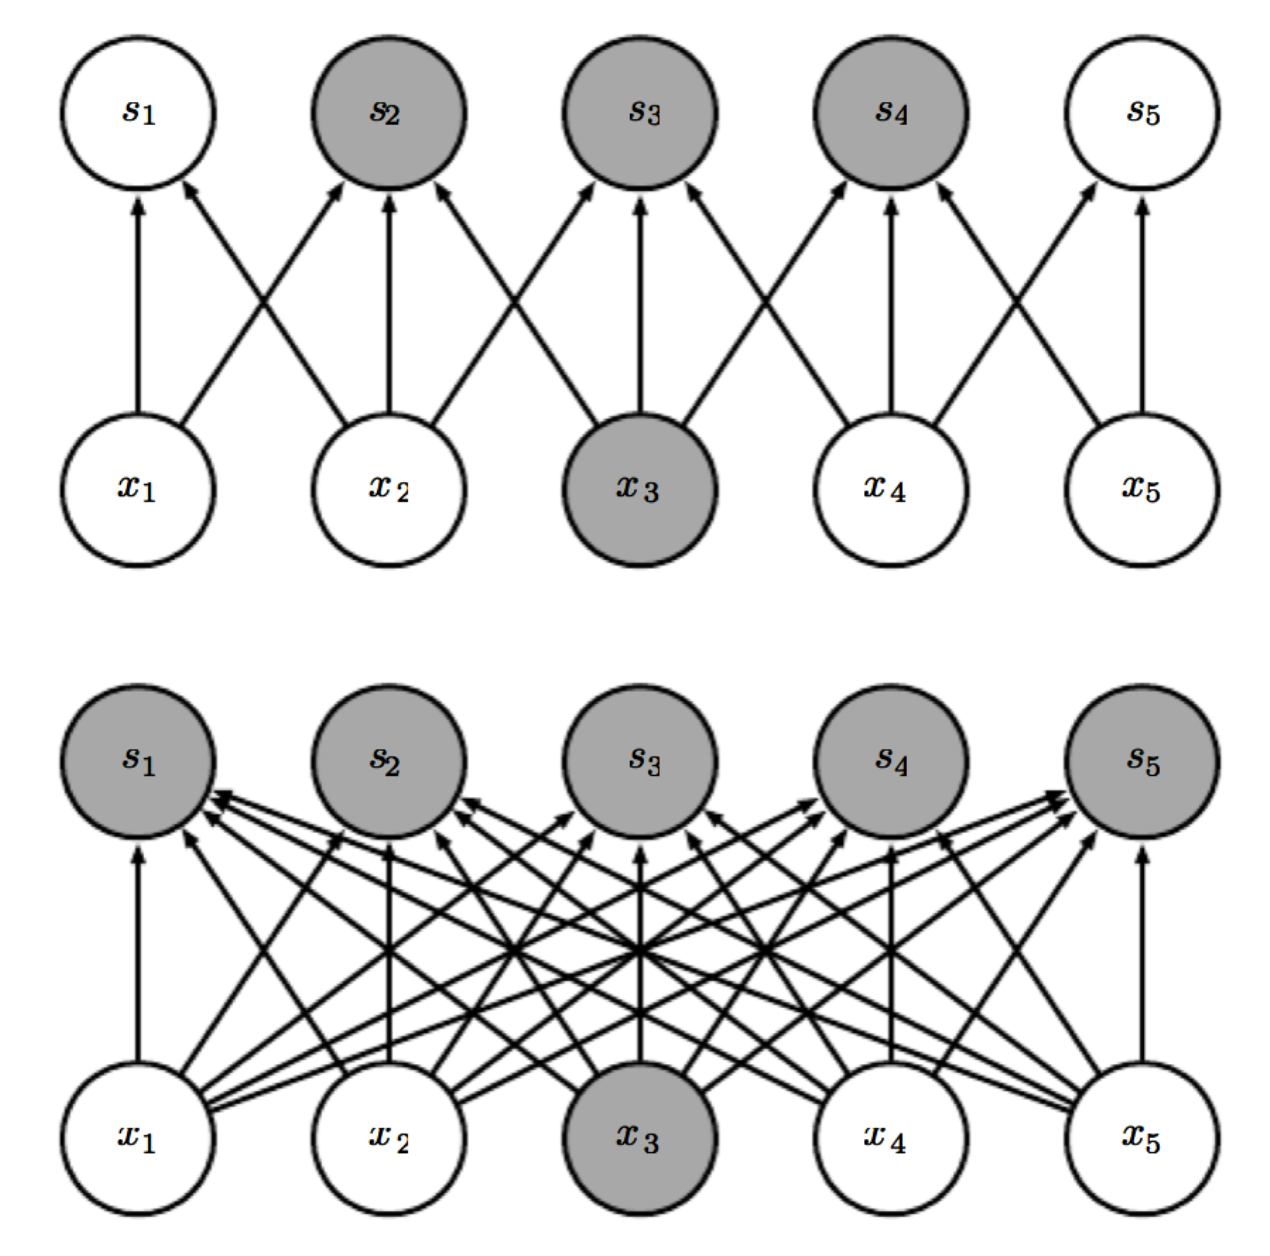
\includegraphics[width=0.5\textheight]{figs/weights-sharing1}
		
		{\small [from \emph{Deep Learning}, Goodfellow, Bengio and Courville]}
	\end{center}
	\begin{itemize}
		\medskip 
		
		\item Top: in a convolution with a kernel of width 3, only three outputs are affected by the input $x$. We say that the \textbf{connectivity is sparse} 
		
		\medskip 
		
		\item Bottom: when using matrix multiplication, all outputs are connected to an input. We say that \textbf{connectivity is dense}
	\end{itemize}
\end{frame}



\subsection{Pooling layer}

\begin{frame}
	\frametitle{Pooling}
	
	The Pooling Layer operates independently on every depth slice of the input and resizes it spatially, using the $\max$ function. 
	
	\begin{center}
		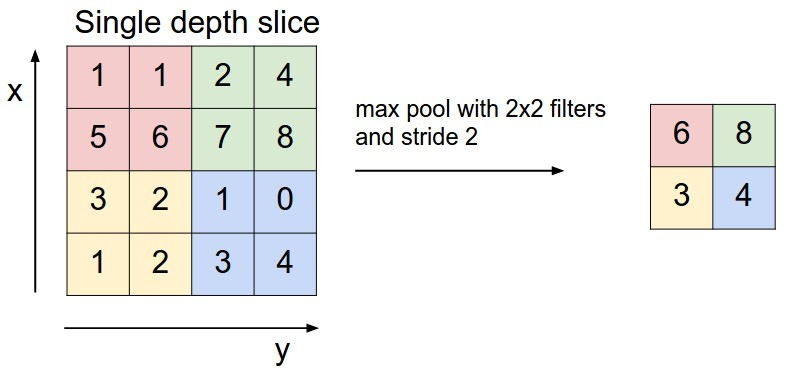
\includegraphics[scale=0.3]{figs/maxpool}
	\end{center}

Parameters: 
\begin{itemize}
	\item Stride $S$
	\item Spatial extend $F$
\end{itemize}

Usually, $S=F=2$ and more rarely $F=3, S=2$ (overlapping pooling).
\end{frame}

\begin{frame}{Pooling}
	\begin{itemize}
		\item Pooling replaces the output at a certain location by a summary statistic of neighboring outputs
		
		\medskip 
		
		\item The most widely used is the \structure{max aggregation}, called \structure{max-pooling}
		
		\medskip 
				
		\item Pooling helps the representation to become \structure{approximately invariant} to small translations of the input
		
		\medskip 
				
		\item If a small translation is applied, output of the layer is almost unchanged
		
		\medskip 
				
		\item Very useful is we care more about the presence of some feature than its position in the image: for face detection (presence of eyes is more important than where they are)
		
		\medskip 
				
		\item   Pooling also allows to handle inputs with different sizes: pictures can have different sizes, but the output classification layer must be of fixed size
	\end{itemize}  
\end{frame}


\begin{frame}
	\frametitle{Convolutional Neural Network}
	
Typically, one or more convolutional layers are followed by one pooling layer and so on. At the end of the network, several fully connected layers are typically used to compute probabilities. 

\begin{center}
	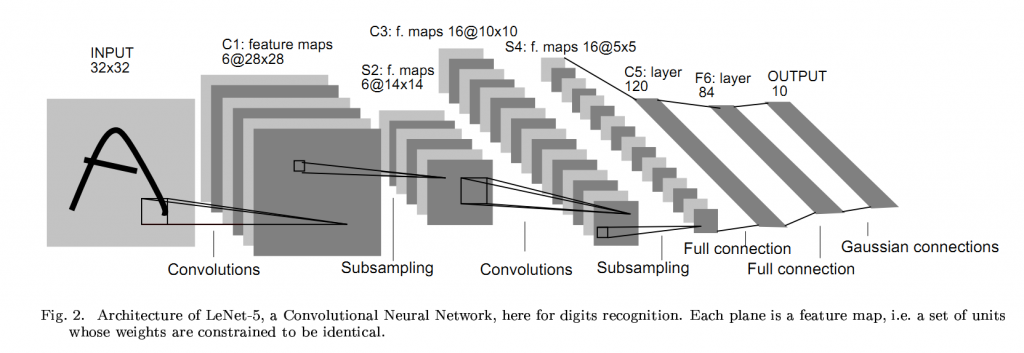
\includegraphics[scale=0.3]{figs/LeNet}
\end{center}
\end{frame}


\subsection{Data preprocessing}

\begin{frame}
	\frametitle{Data processing}
	
	\blue{Normalizing data}
	
	For each channel R, G, B, compute the pixels mean over all images in the whole data set. Substract this value to each channel of each image. 
	$\rightarrow$ you do not lose relative information between images. 
	
	\bigskip
	
	\blue{Data augmentation}
	\begin{enumerate}
		\item Sampling 
		\citem{russakovsky2015imagenet}
		\item Translation/shifting 
		\citem{salamon2017deep}
		\item Horizontal reflection/mirroring 
		\citem{yang2015mirror}
		\item Rotating 
		\citem{xie2015holistically}
		\item Various photometric transformations
		 \citem{eigen2015predicting}
	\end{enumerate}
	
	\blue{Prediction} 
	
	At test time, patches are extracted from the new images together with some of its reflection/translation/... A prediction is made for each of these artificial images and they are aggregated to make the final prediction. 
	
\end{frame}



\begin{frame}
	\frametitle{Adding noise - Data augmentation and regularization}
	

	\begin{itemize}
		\item Add noise to input 
		
		\smallskip 
		
		\citem{bishop1995training}
		
		\smallskip
		
		\citem{rifai2011adding}
		
		\medskip 
		
		\item Add noise to weights
		
		\smallskip
		
		\citem{jim1996analysis}
		
		\smallskip
		
		\citem{graves2011practical}
		
		\medskip 
		
		\item Add noise to output 
		
		\smallskip
		
		\citem{goodfellow2014explaining}
		
		\medskip 
		
		\item Select the best data transformations (computationally expensive, many re-training steps). 
		
		\smallskip
		
		\citem{paulin2014transformation}
	\end{itemize}
	
\end{frame}




\section{Famous CNN}

\subsection{LeNet (1998)}

\begin{frame}
	\frametitle{LeNet}

\citem{lecun1989generalization}

\citem{lecun1998gradient}

\begin{center}
	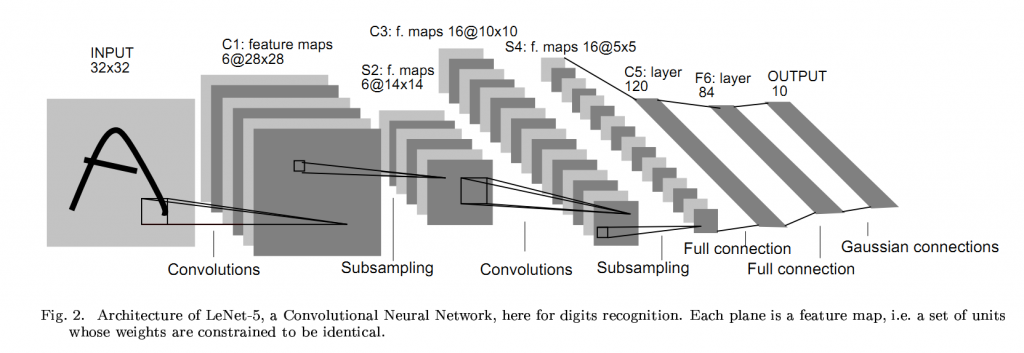
\includegraphics[scale=0.3]{figs/LeNet}
\end{center}

 
First layer: convolutional layer C1
\begin{itemize}
	\item Kernel size = $5 \times 5$ + a bias
	\item Stride = 1 (overlapping contiguous receptive fields)
	\item Zero-padding = 0
	\item Output: 6 different feature maps, each one resulting from the convolution with a kernel $5\times 5$ to which the activation function $\sigma$ is applied. 
\end{itemize}
\end{frame}


\begin{frame}
	 
	
Second layer: subsampling/pooling layer S2
\begin{itemize}
	\item Type of pooling: averaging.
	\item Kernel size = $2 \times 2$
	\item Stride = 2 (non-overlapping receptive fields)
	\item Zero-padding = 0
	\item Output: one feature map per input feature map resulting from the operation
	$\sigma ( (2 \times 2~ \textrm{averaging}) w + b).$
\end{itemize}

\bigskip 

Third-layer: convolutional layer C3
\begin{itemize}
	\item Warning: this layer operates on several feature maps whereas layer C1 operates on the input image (depth = 1).
	\item Here each feature map is connected to some specific input feature maps in order to 
		 
	\begin{itemize}
		\item Reduce the number of connections
		\item Break the symmetry between the different layers of the network. 
	\end{itemize}

\begin{center}
	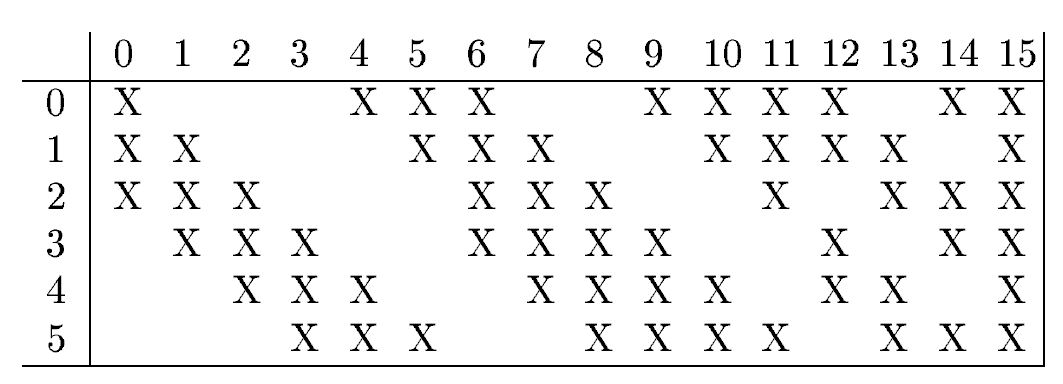
\includegraphics[scale=0.3]{figs/Lenet_connections_third_layer}
\end{center}


\end{itemize}
\end{frame}

\begin{frame}
	\frametitle{What about the remaining layers}
	
	\begin{center}
		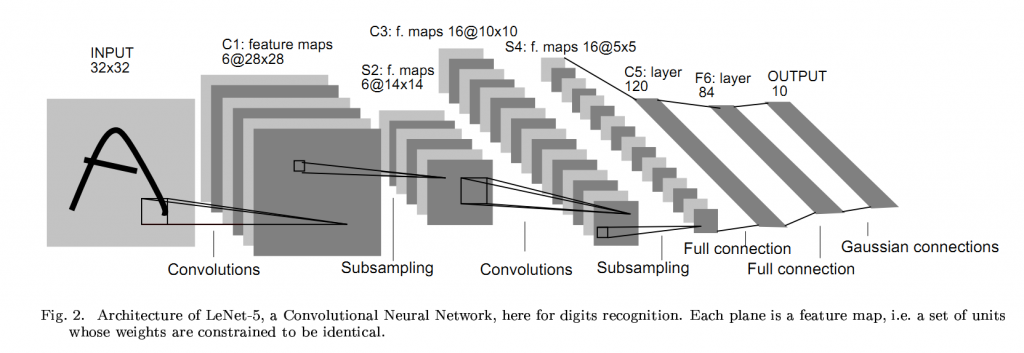
\includegraphics[scale=0.3]{figs/LeNet}
	\end{center}

\pause 
\begin{itemize}
	\item S4: Pooling layer as before
	\item C5: Convolutional layer connected to all previous feature maps. 
	\item F6: fully-connected layer with $84$ units
	\item Output: a specific layer
\end{itemize}

\blue{Bi-pyramidal structure}: the number of feature maps increases while the spatial resolution decreases. 
	
\end{frame}

\begin{frame}
	\frametitle{Output layer}
	
	
	
	Radial Basis function units:
	\begin{itemize}
		\item the parameters of neuron $j$ of the output layer are $w_j = (w_{j,1}, \hdots , w_{j, 84})$.
		
		\item the neuron $j$ outputs
		$$
		\|x - w_j\|_2^2 = \sum_{i=1}^{84} (x_i - w_{j,i})^2,
		$$
		where $x$ is the input vector of size $84$. 
	\end{itemize}
	
	\bigskip
	
	Assuming that the vector in layer F6 are Gaussian, neuron $j$ outputs the negative log likelihood of a Gaussian distribution with mean $w_j$ and covariance matrix $I$.
	
	\bigskip
	
	In other words, each neuron outputs the square euclidean distance between its parameter vector and the input.
	
	\medskip  
	
	How to choose $w_j \in \{-1, 1\}^{84}$?
	 
\end{frame}

\begin{frame}
	\frametitle{Output layer and activation function}
	
	To choose $w_0 \in \{-1, 1\}^{84}$, use a stylized version of the image of $0$ of size $7\times 12 =84$. The pixel of this image are the parameters $w_j$ of the output neuron $j=0$. 
	
	\medskip 
	
	\blue{Why do not use a one-hot encodage?}
	\smallskip
	
	\cite{lecun1998gradient} states that it does not work with more than few dozens of classes since it requires output units to be off most of the time which is difficult to achieve with sigmoid functions. 
	
	\bigskip
	
	
	\begin{block}{Activation function}
	$$\sigma(x) = A \tanh (\alpha x),$$
	where $A = 1.7159$, $\alpha=2/3$. 
	\end{block}
	
	\smallskip 
	
	$\rightarrow$ \blue{Prevent saturation} since neurons outputs belong to $\{-1, 1\}$
	\begin{itemize}
		\item $\sigma(1) = 1$
		\item $\sigma(-1) = -1$.
	\end{itemize}
	
\end{frame}

\begin{frame}
	\frametitle{Criterion to optimize}
	
	Error for one observation $(x_i, y_i)$: 
	$$
	E (\theta) = \sum_{k=0}^{9}  [f_{\theta}(x_i)]_k \mathds{1}_{y_i = k}
	+ \log \Big(e^{-C} + \sum_{k=0}^9 e^{- [f_{\theta}(x_i)]_k} \Big),
	$$
	where $[f_{\theta}(x_i)]_k$ is the output of the output neuron $k$, $C>0$ is a constant. 
	
	\medskip 
	
	The second term acts as a regularization since it forces the parameters of the neurons $k\neq y_i$ to be far from the input vector of layer F6.
	
	\pause 
	\bigskip
	
	This is equivalent to 
	$$
	E (\theta) = - \log \Big( \frac{e^{-[f_{\theta}(x_i)]_{y_i}}}{e^{-C} + \sum_{k=0}^9 e^{- [f_{\theta}(x_i)]_k} }\Big),
	$$
	
	\smallskip
	which is very close to the \blue{negative log likelihood of a softmax} output layer. 
\end{frame}

\begin{frame}
	\frametitle{Optimization procedure}
	
	
	
Related to stochastic gradient descent:

	$$
	\theta^{(k+1)}_j = \theta^{(k)}_j - \frac{\eta}{\mu + h_{jj}} \frac{\partial E_i}{\partial \theta_j},
	$$
	
	\smallskip
	where $E_i$ is the loss of a single observation, $\eta$ is the initial learning rate, $\mu$ a hand-picked constant and $h_{jj}$ is the $j$th diagonal element of the Hessian matrix associated to $E_i$. 
	
	\bigskip
	
	The expression of $h_{jj}$ is quite complicated since $\theta_j$ appears in different connections: 
	
	$$
	h_{jj} = \sum_{(i,m) \in V_j} \sum_{(k,l) \in V_j} \frac{\partial^2 E_i}{\partial u_{im} \partial u_{k l}},
	$$
	
	\smallskip
	where $u_{im}$ is the connection between units $i$ and $m$, and $V_j$ is the set of pairs $(i,m)$ such that the connection between $i$ and $m$ involves the weight $\theta_j$.
	
	\bigskip
	
	An approximation of each diagonal terms $h_{jj}$ is performed at the beginning of each epoch, using the first $500$ observations (whole data set being composed of $60000$ observations).
	
	\end{frame}

\begin{frame}
	\frametitle{Parameters}
	
	Weight initialization: uniform distribution $U([-2.4/F_i, 2.4/F_i])$, where $F_i$ is the number of inputs (fan-in) of the unit which the connection belongs to. 
	
	\smallskip
	
	$\rightarrow$ Keep the weighted sum in the same range for each unit. 
	
	\bigskip
	
	
	\begin{block}{Gradient descent}
	$$
	\theta^{(k+1)}_j = \theta^{(k)}_j - \frac{\eta}{\mu + h_{jj}} \frac{\partial E_i}{\partial \theta_j},
	$$
	with $\mu = 0.02$. 
	\end{block}


	\bigskip

	Optimization lasts 	$20$ epochs: 
	\begin{itemize}
		\item $\eta = 0.0005$ for the first two epochs,
		\item $\eta = 0.0002$ for the next three epochs,
		\item $\eta = 0.0001$ for the next three epochs,
		\item $\eta = 0.00005$ for the next four epochs,
		\item $\eta = 0.00001$ for the remaining epochs,
	\end{itemize}
	
	
	

	
	
	
\end{frame}




\begin{frame}
	\frametitle{Results}
	
	\begin{center}
		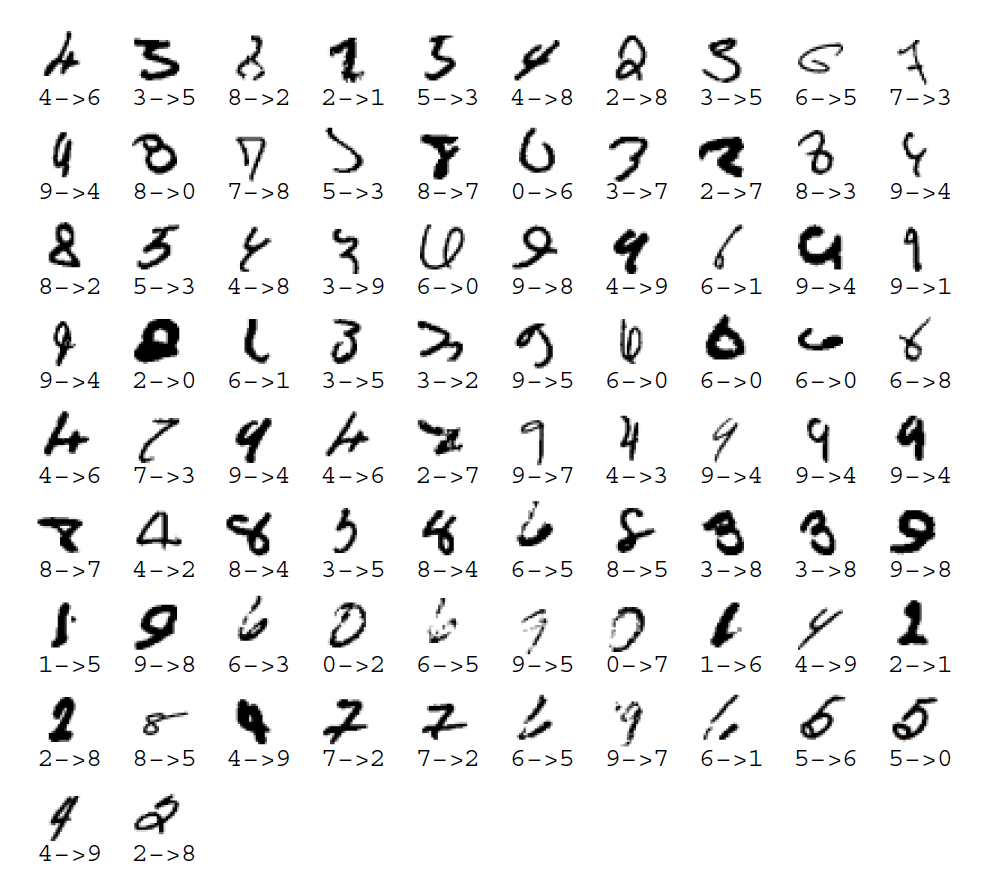
\includegraphics[scale=0.5]{figs/Lenet_misclassified_digits}
	\end{center}

{\small The $82$ patterns misclassified by LeNet5. Below each image is displayed the correct answer (left) and the prediction (right). These errors are mostly caused by genuinely ambiguous patterns, or by digits written in a style that are under represented in the training set.} 
\end{frame}











\subsection{AlexNet (2012)}

\begin{frame}
	\frametitle{AlexNet}
	
	\citem{krizhevsky2012imagenet}
	
	\bigskip
	
	 Ingredients: 
	 \begin{itemize}
	 	\item Activation function (ReLU)
	 	\item Local Response Normalization (LRN)
	 	\item Overlapping pooling
	 	\item Dropout
	 	\item Data augmentation
	 \end{itemize}
 
 \bigskip
 
\begin{center}
	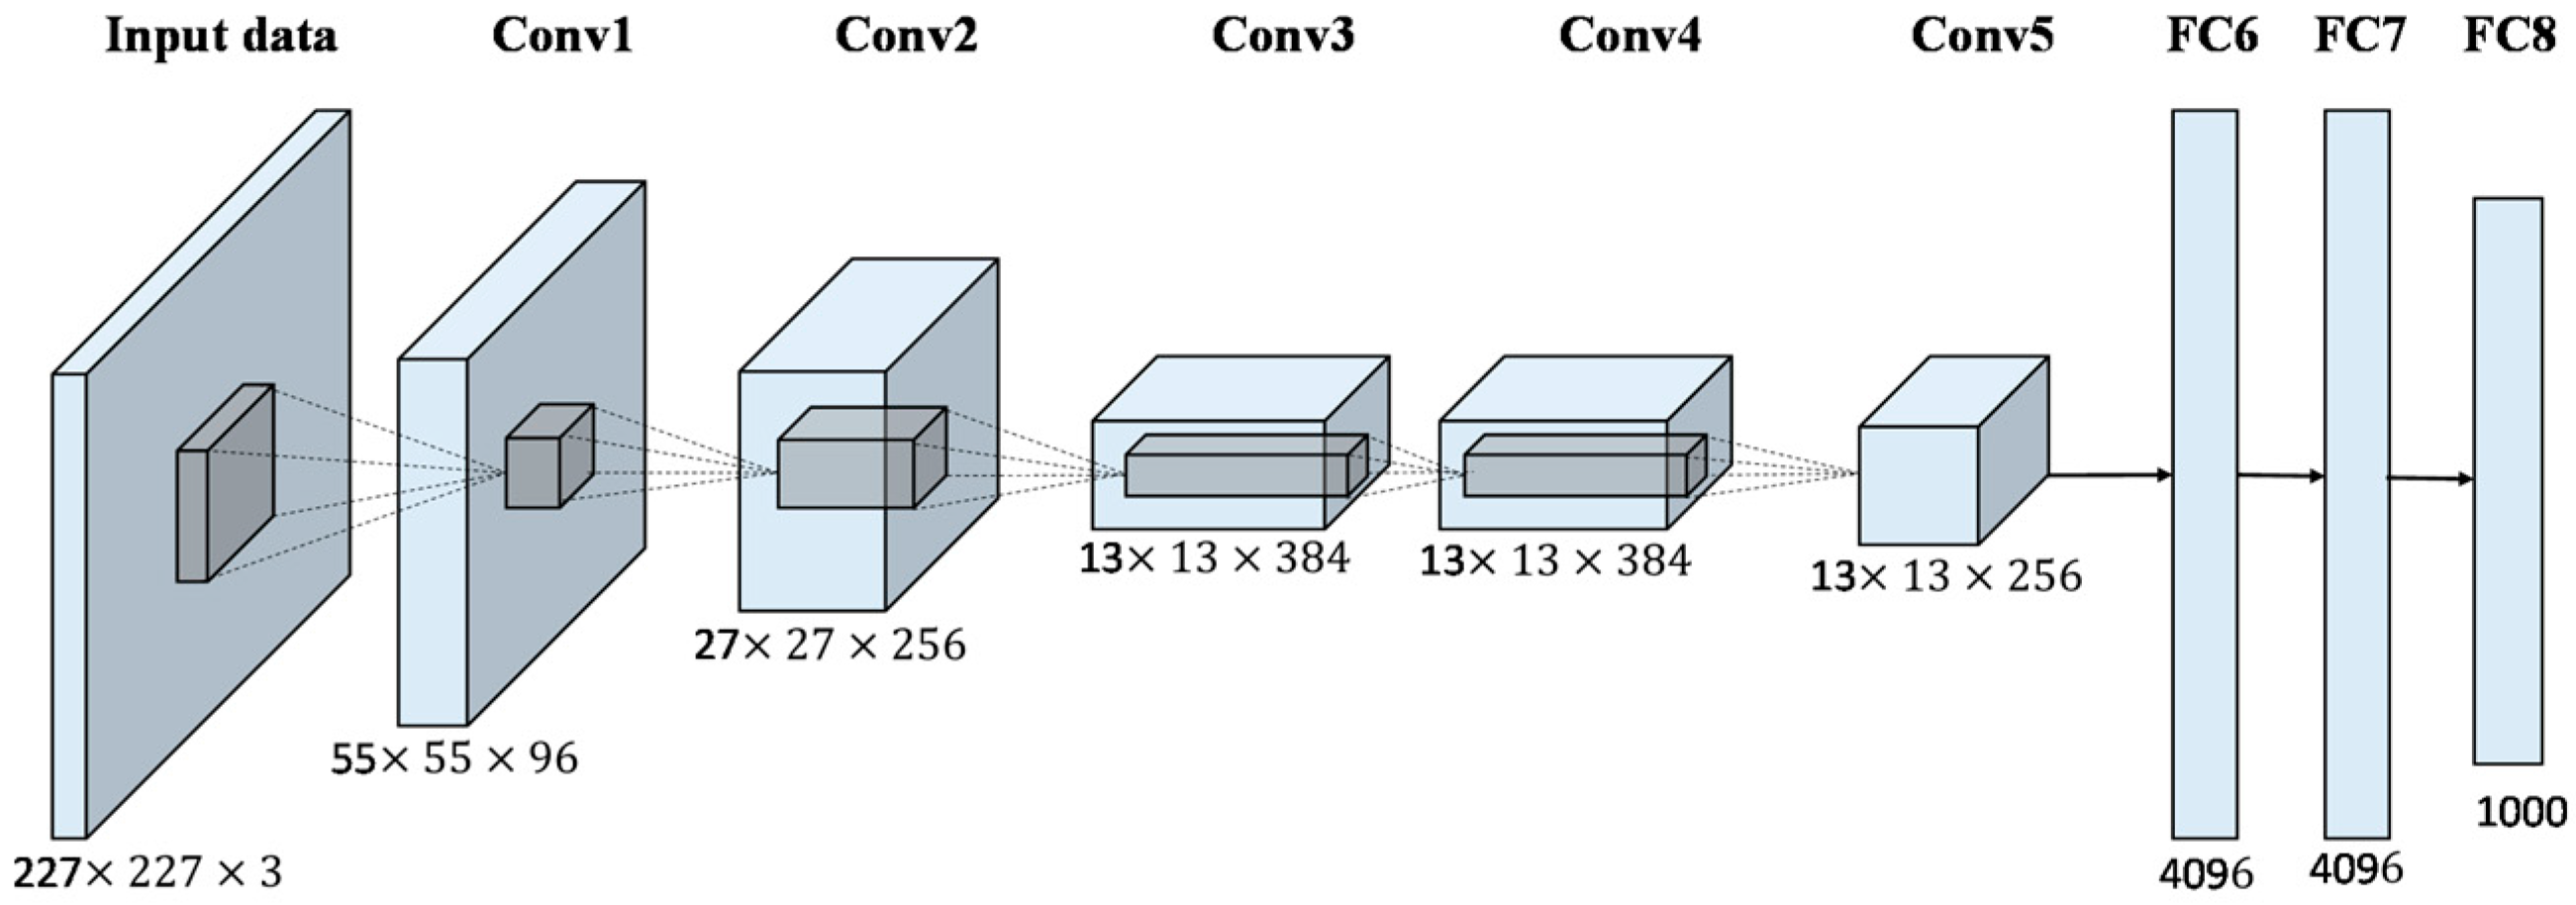
\includegraphics[scale=0.6]{figs/AlexNet}
\end{center}

\end{frame}

\begin{frame}
	\frametitle{ReLU activation function}
	
	According to \cite{krizhevsky2012imagenet}, Convolutional neural networks with ReLU activation functions can be trained several times faster than the same networks using $\tanh$ function. 
	
	\medskip
	
	\begin{center}
		\begin{figure}
		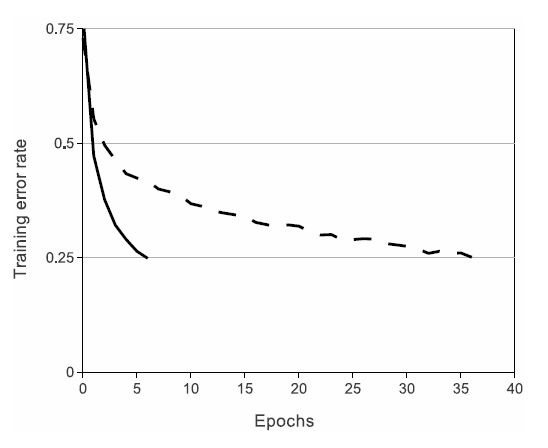
\includegraphics[scale=0.75]{figs/Alexnet_reluVsTanh}
		\caption{A four-layer convolutional neural network with ReLU (solid line) reaches a $25\%$ training error rate on CIFAR-10 six times faster than an equivalent network with $\tanh$ (dashed line). The learning rates for each network were chosen independently to make training as fast as possible.}
		\end{figure}

	\end{center}

\end{frame}


\begin{frame}
	\frametitle{Local Response Normalization/ Brightness normalization}
	
	

	Let $a_{x,y}^i$ the activity of a neuron resulting of kernel $i$ applied to the position $(x,y)$ followed by a ReLU function and $b_{x,y}^i$ the corresponding renormalized activity which is given by
	
	$$
	b_{x,y}^i = a_{x,y}^i \Bigg( C + \alpha \sum_{j = \max(0, i - q/2)}^{\min(Q-1, i + q/2)} (a_{x,y}^j )^2 \Bigg)^{-\beta},
	$$
	
	\smallskip
	
	where the sum is taken over $q$ adjacent feature maps at the same spatial position, and $Q$ is the total number of feature maps in this layer. 
	
	\smallskip
	
	Constants (determined with validation set): $C=2, q=5, \alpha = 10^{-4}, \beta = 0.75$.
	
	\bigskip 
	
	Note that the ordering of feature maps is arbitrary and determined before training. This renormalization creates a competition between the different feature maps. 
	
	\bigskip
	\citem{jarrett2009best}
	
	\smallskip 
	
	They propose a similar normalization procedure where the mean activity is substracted (local contrast normalization).
	
\end{frame}

\begin{frame}
	\frametitle{Overlapping pooling}
	
	Usually receptive fields in pooling layers do not overlap. Here, they use a grid of size $3 \times 3$ with a stride $s=2$. Resulting network is slightly less prone to overfitting.
	
	\medskip
	
	\begin{center}
		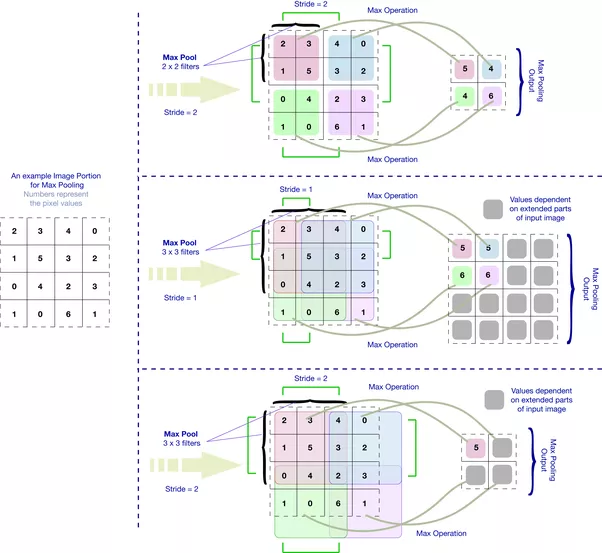
\includegraphics[scale=0.38]{figs/pooling_overlapping}
	\end{center}

\medskip

$\rightarrow$ 
	
\end{frame}



\begin{frame}
	\frametitle{Overall architecture}
	
	
	
	\begin{center}
		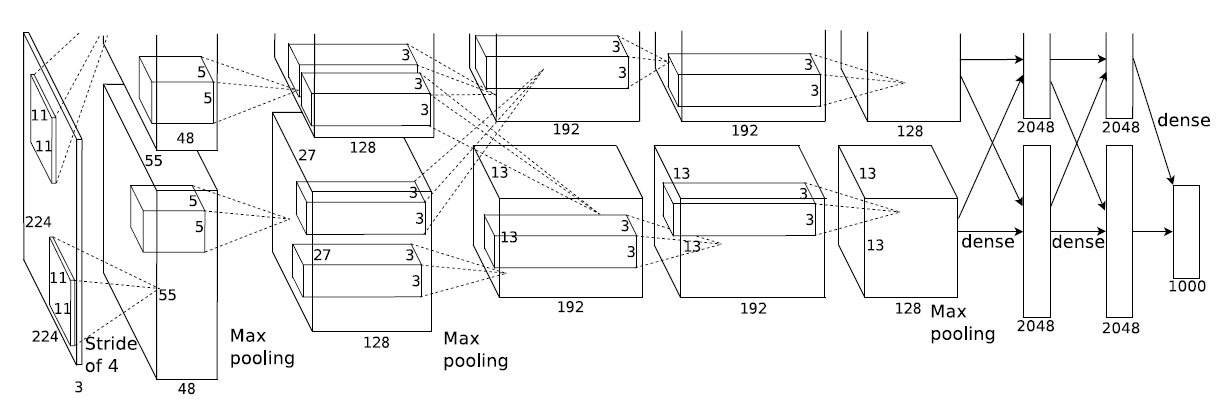
\includegraphics[scale=0.6]{figs/AlexNet_twoGPU_architecture}
	\end{center}
	
	Key-point: architecture is split across two GPU, which, most of the time, do not communicate with each other.
	
	\begin{itemize}
		\item Connectivity of each convolutional layer
		\item ReLu are applied right after all convolutional layers and fully connected layers
		\item Local Response Normalization is applied after ReLU in the first and second convolutional layer
		\item Max-pooling is applied after the first, second and fifth convolutional layers.
	\end{itemize}
	
	
	
\end{frame}

\begin{frame}
	\frametitle{Parameters}
	
	Initialization: 
	\begin{itemize}
		\item Weights: $\mathcal{N}(0, 0.0001)$
		\item Biases of second, fourth and fifth convolutional layers and biases of fully connected layers set to $1$ (seems to accelerate the early stages of learning: nonzero ReLU output). 
		\item Other biases are set to $0$
	\end{itemize}



	
	\begin{block}{Stochastic gradient descent with momentum}
	\begin{align*}
	v^{(k+1)} & = 0.9 v^{(k)} - 0.0005 \eta \theta^{(k)} - \frac{\eta}{B} \sum_{i \in \mathcal{B}} \nabla \ell_i (\theta^{(k)})\\
	\theta^{(k+1)} & = \theta^{(k)} + v^{(k+1)},
	\end{align*}	
	with batch size $|\mathcal{B}| = B = 128$. 
	\end{block}



Learning rate is the same for all layers with the following heuristic: 
\begin{itemize}
	\item Initialization: $\eta = 0.01$
	\item Divide $\eta$ by $10$ when the validation error stop improving
	(this has been done three times).
	\item $90$ epochs on $1.2$ million images: 6 days.
\end{itemize}


\end{frame}

\begin{frame}
	\frametitle{Numerical results}
	
	\begin{center}
		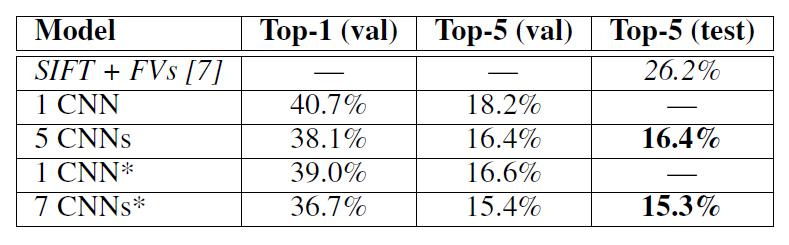
\includegraphics[scale=0.6]{figs/Alexnet_error}
	\end{center}



\bigskip

\begin{itemize}
	\item First line is the second runner-up.
	
	\item Second and third lines are results output by the averaging over $1$ or $5$ CNN described before. 
	
	\item Last two lines correspond to networks with an extra convolutional layer after the last pooling layer which has been trained on Image Net Fall 2011 then ``fine-tuned'' on the ImageNet 2012 data base. 
\end{itemize}


\bigskip

AlexNet has a very similar architecture to LeNet, but is deeper, bigger, and features Convolutional Layers stacked on top of each other: previously, pooling layers followed immediately each convolutional layer. 

\end{frame}



\begin{frame}
	\frametitle{Results}
	
	\begin{center}
		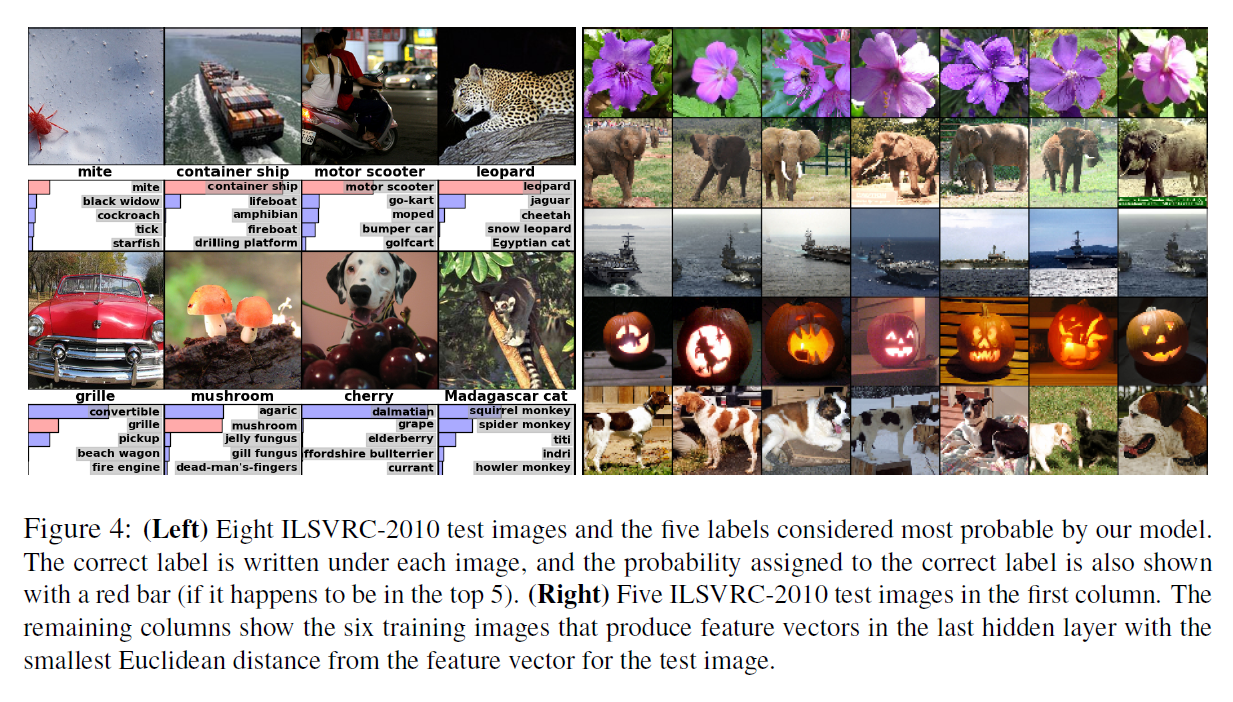
\includegraphics[scale=0.7]{figs/AlexNet_results_images}
	\end{center}
\end{frame}








\subsection{ZFNet (2013)}

\begin{frame}
	\frametitle{ZFNet: Improve upon AlexNet}
	
	\citem{zeiler2014visualizing}
	
	\bigskip
	
	\begin{center}
		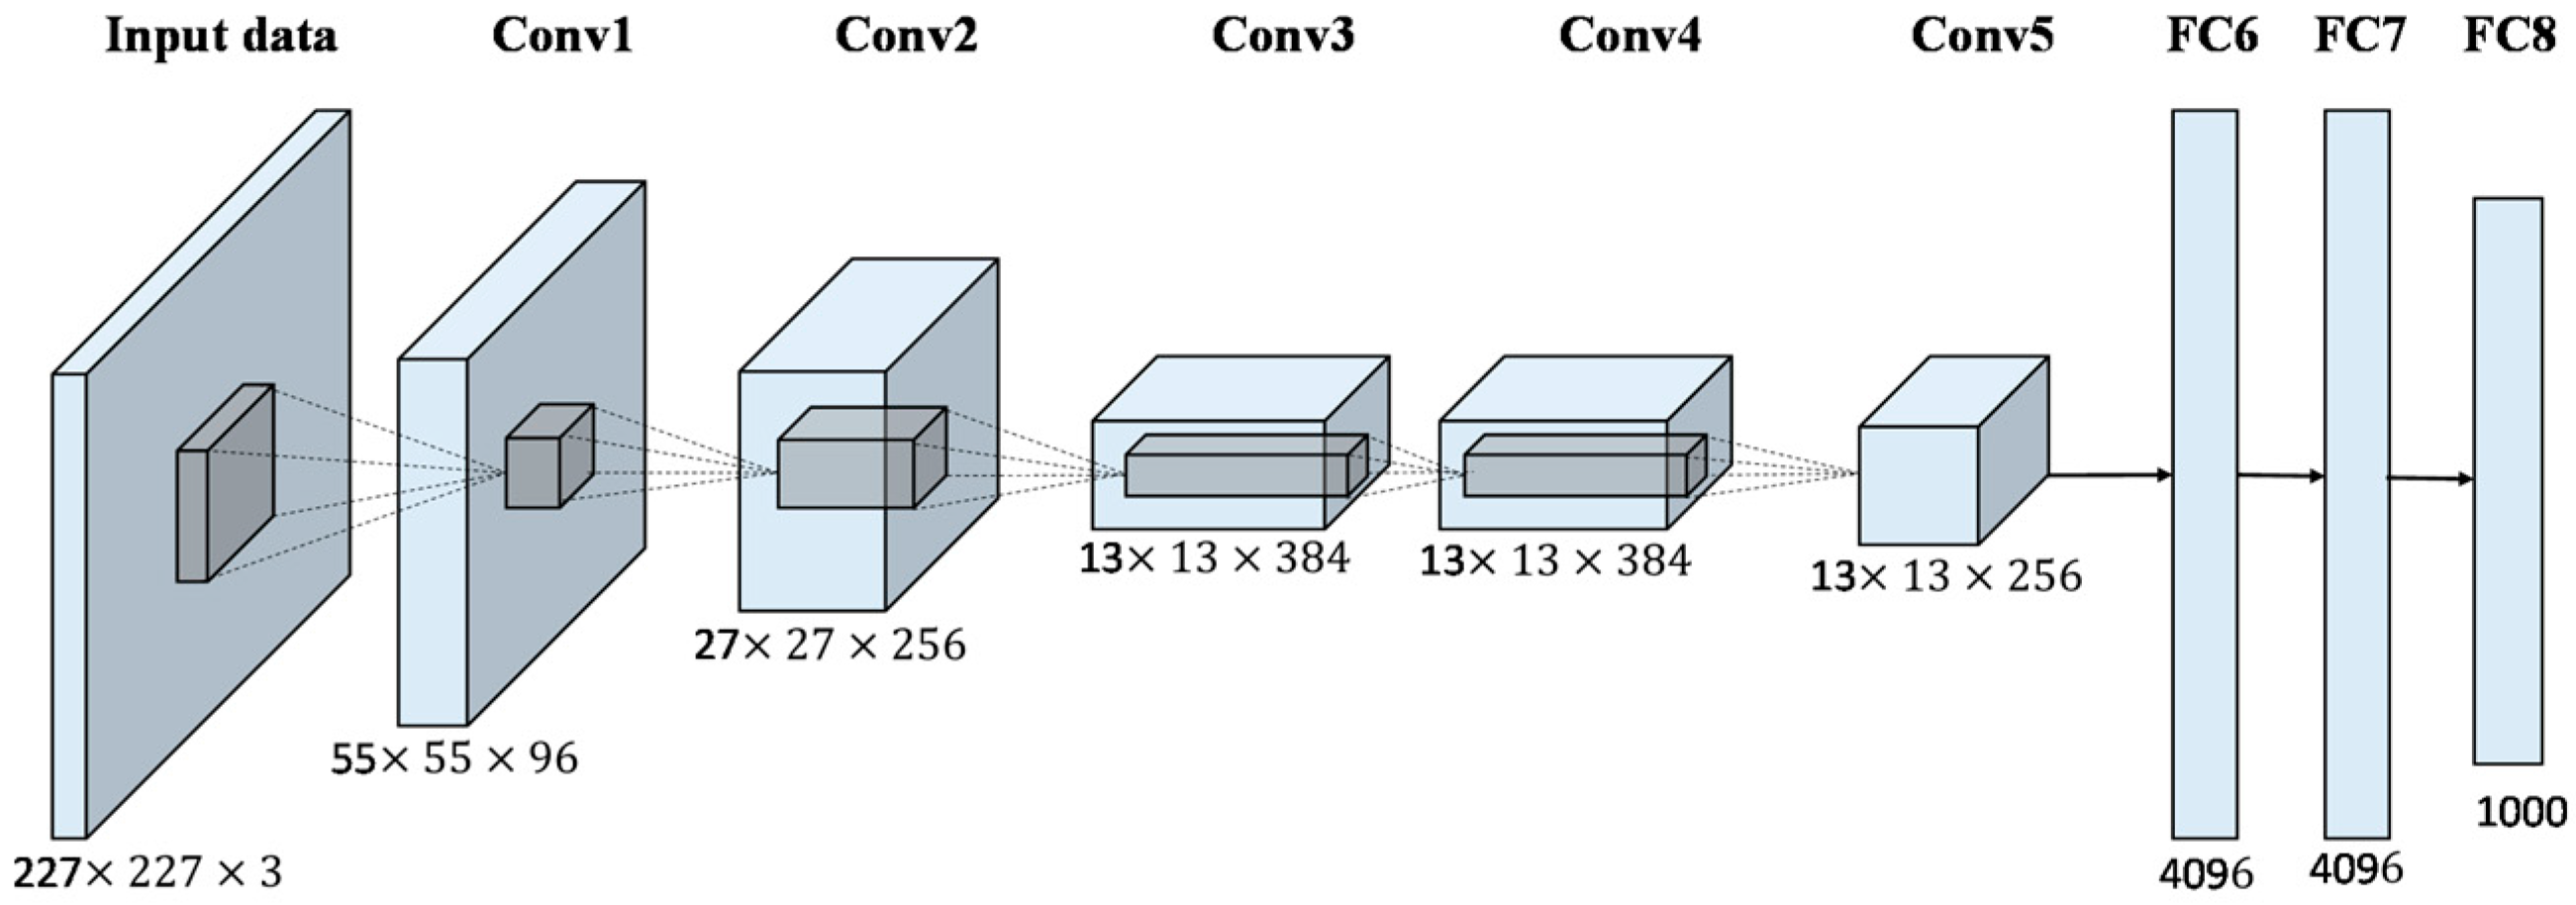
\includegraphics[scale=0.6]{figs/AlexNet}
	\end{center}

	\bigskip

	Aim at finding out \blue{what the different feature maps are searching for} in order to obtain a better tuning of network architecture. 
	
	\bigskip
	
	In ZFNet, feature maps are not divided across two different GPU. Thus connections between layers are \blue{dense}. 
\end{frame}

\begin{frame}
	\frametitle{Deconvnet}
	
		
	\begin{columns} % align columns
		\begin{column}{.4\textwidth}
		Find the pixels that maximize the activation of a given feature map.
			 
		\bigskip 
		
		How? Invert the network.
		
		\bigskip 
		
		Precisely: 
		\begin{itemize}
			\item Choose a layer
			\item Choose a feature map
			\item Run the network on a validation set
			\item Choose the image maximizing the activation of this feature map
			\item "Backpropagate" this activation to obtain a stylized image in the pixel space
		\end{itemize}	
		\end{column}%

		\begin{column}{.6\textwidth}
			\hspace{-1.5cm}
			\begin{center}
				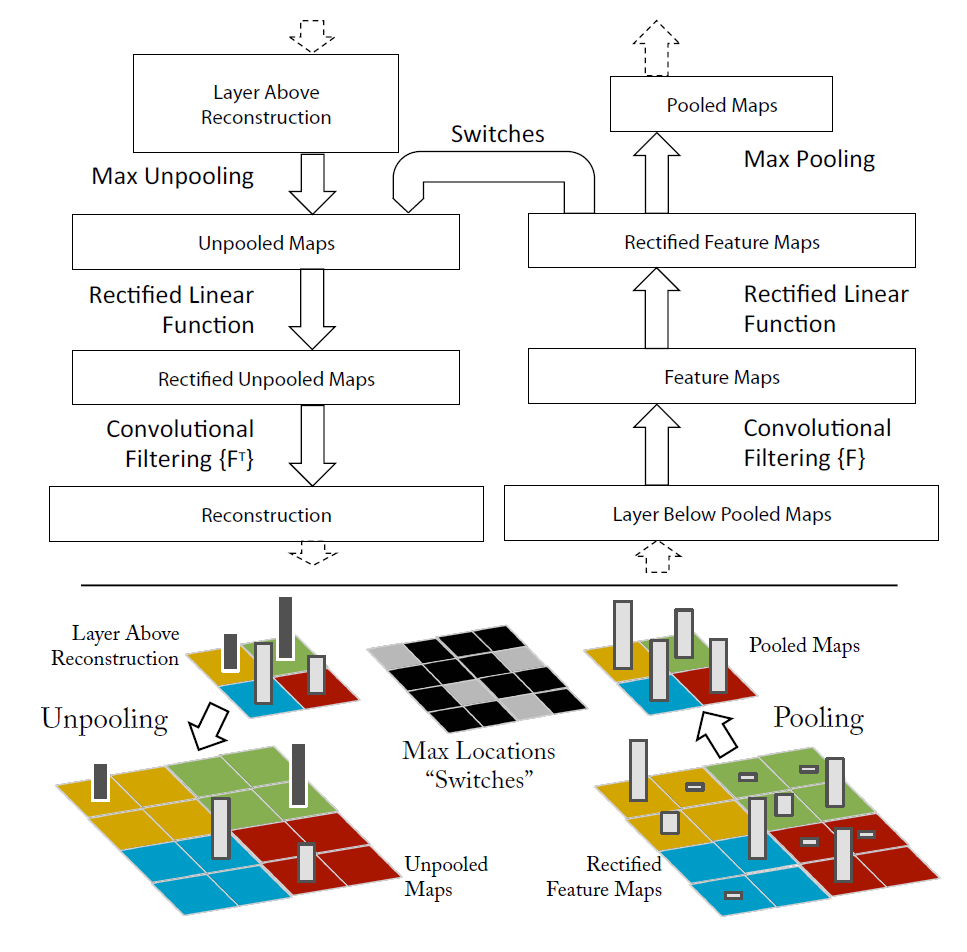
\includegraphics[scale=0.6]{figs/deconvnet}
			\end{center}
		\end{column}%
	\end{columns}
	
	
 
	
	
	
\end{frame}

\begin{frame}
	\frametitle{Results}
	
\begin{center}
	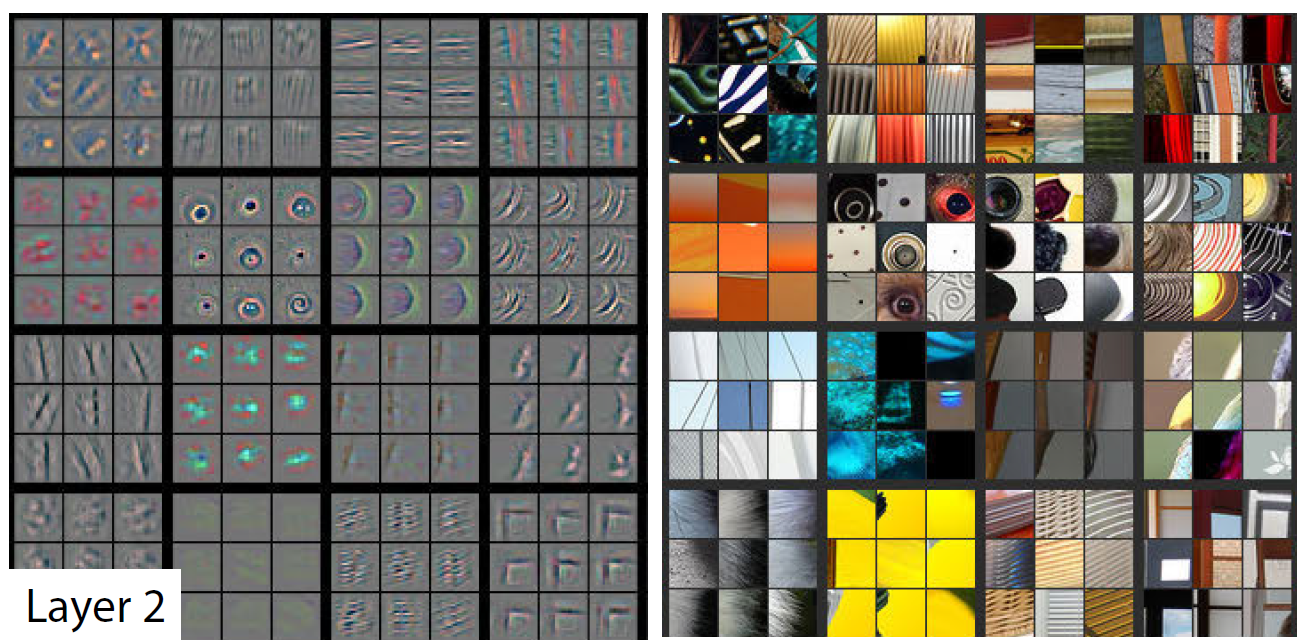
\includegraphics[scale=0.7]{figs/ZFnet_layer2}
\end{center}

Top 9 activations in a random subset
of feature maps across the validation data, projected down to pixel space using our deconvolutional network approach.
\end{frame}

\begin{frame}
	\frametitle{Results}
	
	\begin{center}
		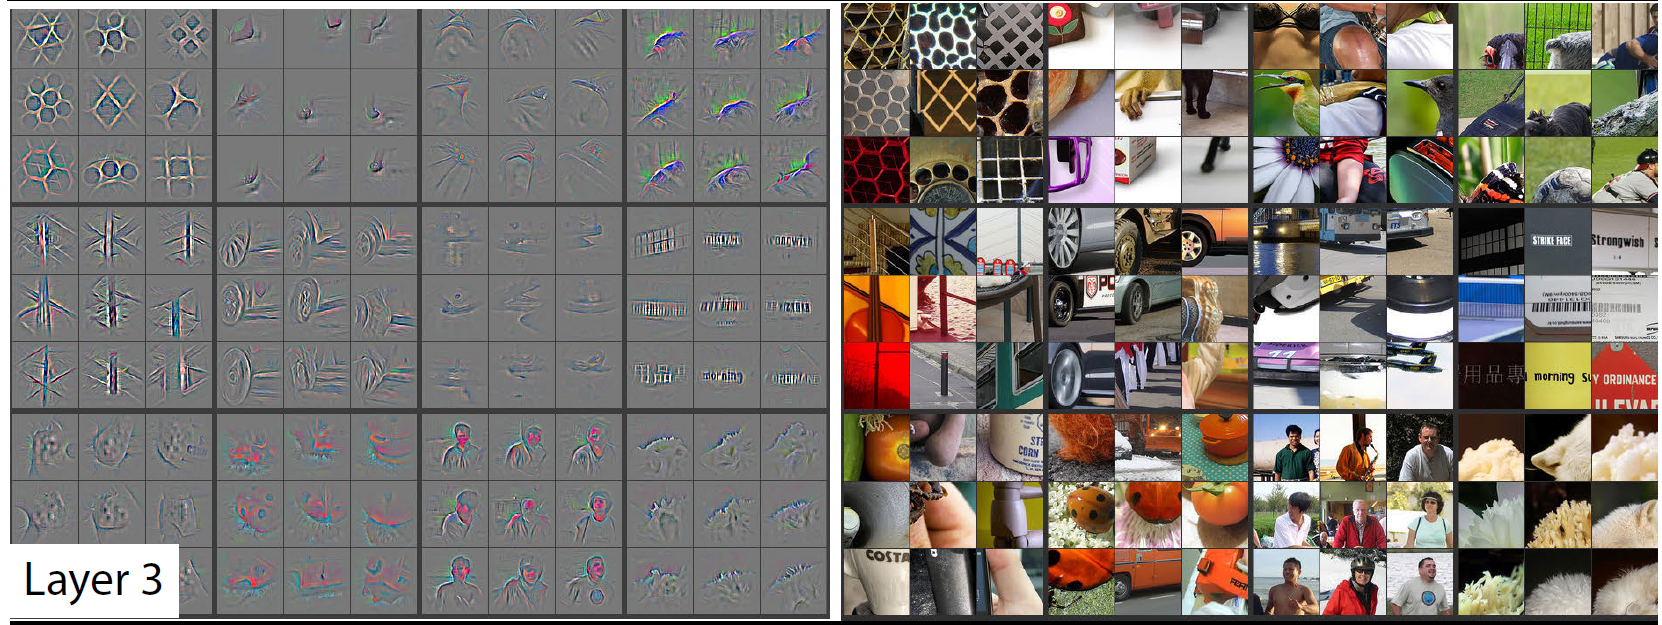
\includegraphics[scale=0.5]{figs/ZFnet_layer3}
	\end{center}
\end{frame}

\begin{frame}
	\frametitle{Results}
	
	\begin{center}
		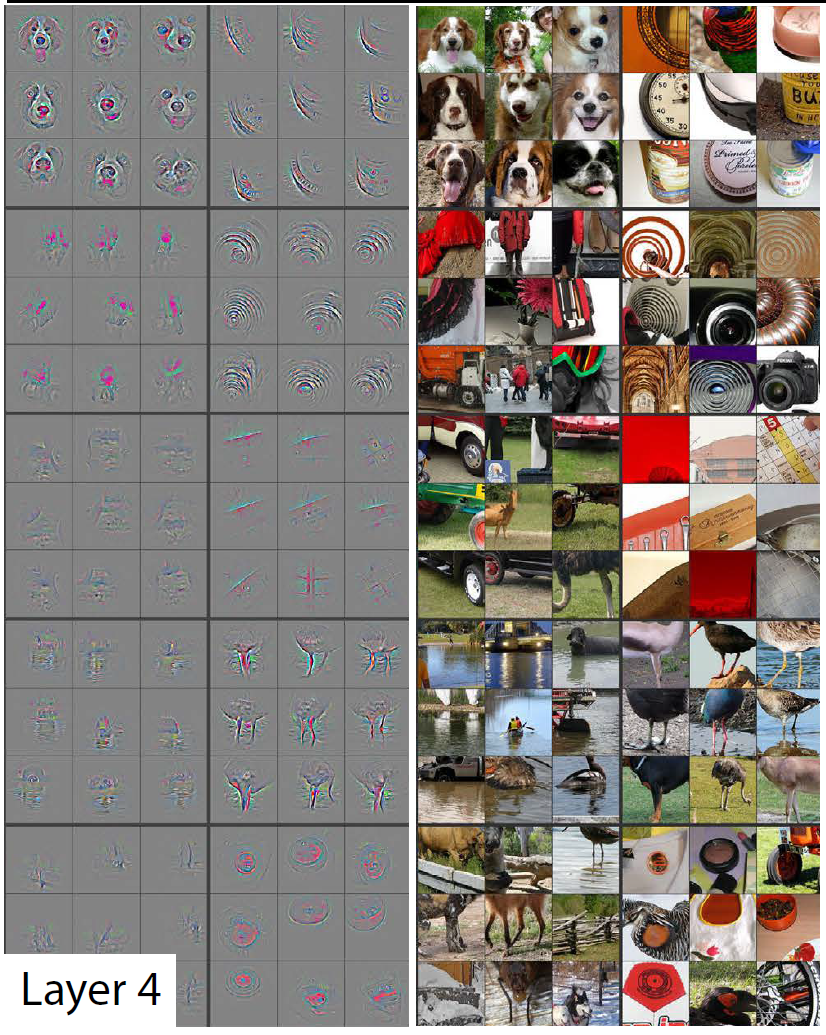
\includegraphics[scale=0.5]{figs/ZFnet_layer4}
	\end{center}
\end{frame}

\begin{frame}
	\frametitle{Results}
	
			
	\begin{columns} % align columns
		\begin{column}{.6\textwidth}
		\begin{center}
			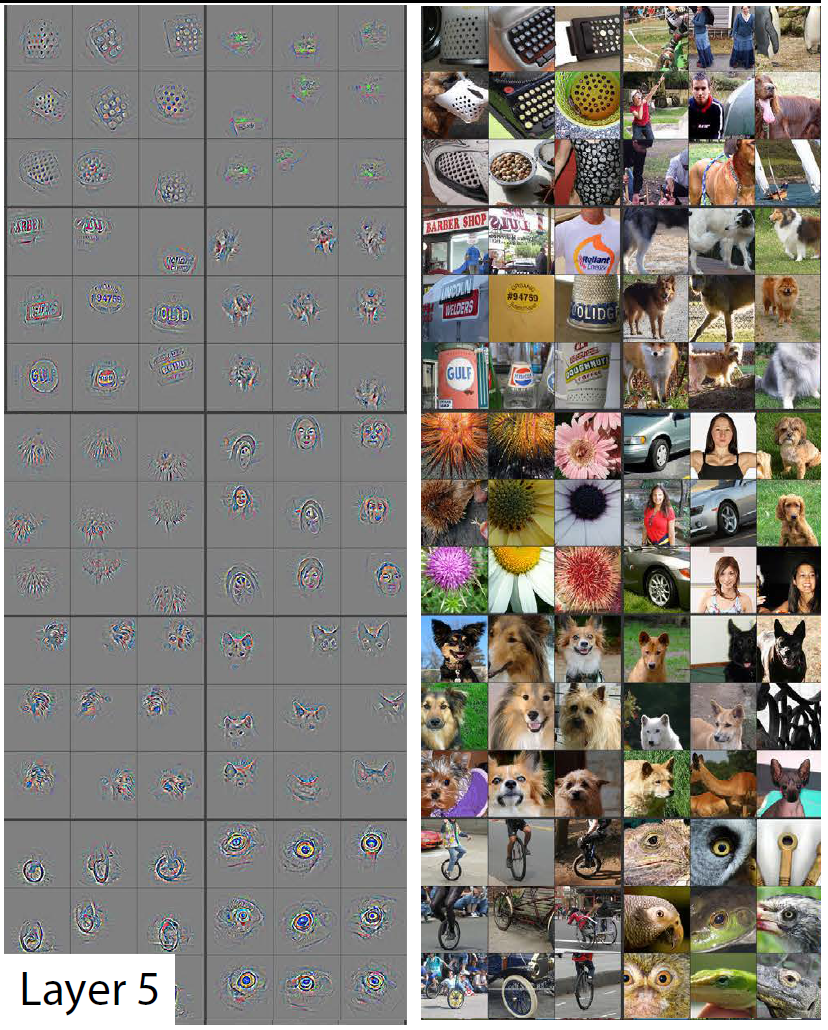
\includegraphics[scale=0.5]{figs/ZFnet_layer5}
		\end{center}	
		\end{column}%
		
		
		
		\begin{column}{.4\textwidth}
			
			\blue{Remarks}
			
			\bigskip 
			
			\begin{itemize}
				\item strong grouping within each feature map,
				
				\medskip 
				
				\item greater invariance at higher layers
				
				\medskip 
								
				\item exaggeration of discriminative parts of the image, e.g. eyes and noses of dogs (layer 4, row 1, cols 1).
				
			\end{itemize}
		\end{column}%
	\end{columns}





\end{frame}

\begin{frame}
	\frametitle{Visualization of previous modifications}
	
		\begin{columns} % align columns
		\begin{column}{.6\textwidth}
			\begin{center}
			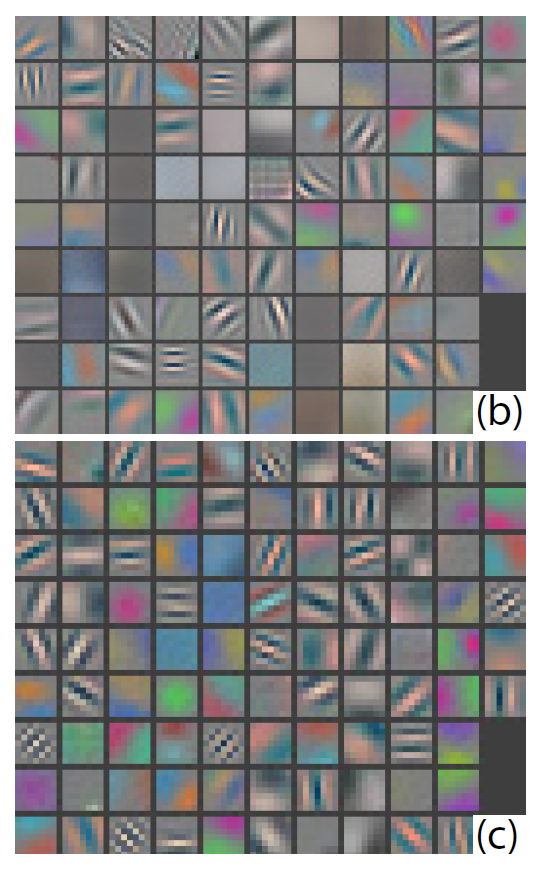
\includegraphics[scale=0.6]{figs/vizualization_cnn}
		\end{center}
		\end{column}%
		
		
		
		\begin{column}{.4\textwidth}
			
		(b): 1st layer features from \cite{krizhevsky2012imagenet}. 
		
		\medskip 
		
		(c): Our 1st layer features. 
		
		\pause 
		
		\bigskip 
		
		The smaller stride (2 vs 4) and filter size (7x7 vs 11x11) results in more distinctive features and fewer dead features. 
		\end{column}%
	\end{columns}
	
	
	
	

	

		
\end{frame}

\begin{frame}
	\frametitle{Visualization of previous modifications}
	
	\begin{center}
		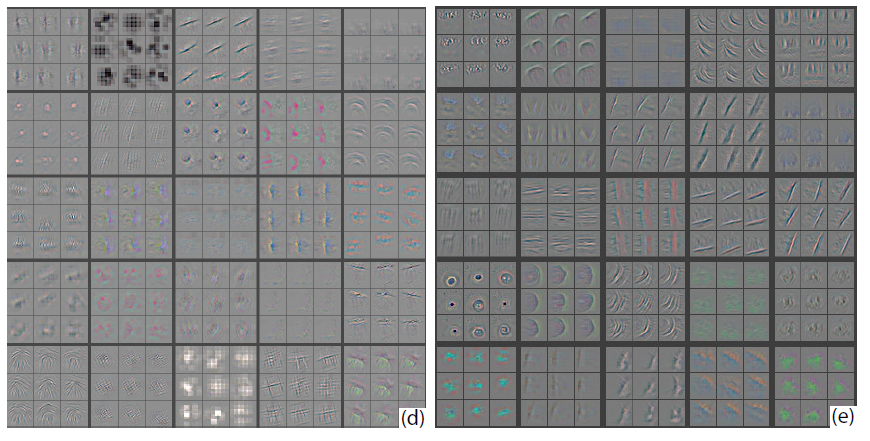
\includegraphics[scale=0.8]{figs/ZFNet_modif_2layer}
	\end{center}
	
	(d): Visualizations of 2nd layer features from \cite{krizhevsky2012imagenet};  (e): Visualizations of our 2nd layer features. 
	
	\pause 
	
	Feature maps in (e) are cleaner, with no aliasing artifacts that are visible in (d).
	
\end{frame}




\begin{frame}
	\frametitle{Conclusion regarding AlexNet}
	
	\begin{itemize}
		\item First layer filters are a mix of high and low frequency information, with little coverage of middle frequencies.
		
		\smallskip
		$\rightarrow$ Reduced the first layer filter size from $11 \times 11$ to $7 \times 7$.
		
		\medskip
		
		\item Aliasing artifacts are present in second layer because of the large stride of $4$ used in the first convolutional layer. 
		
		\smallskip
		$\rightarrow$ change the stride from $4$ to $2$. 
	\end{itemize}

\bigskip

With these modifications: 
\begin{itemize}
	\item Winner of the ILSVRC 2013
	\item Improvement on AlexNet by 
	\begin{itemize}
		\item expanding the size of the middle convolutional layers
		\item making the stride and filter size on the first layer smaller.
	\end{itemize}
\end{itemize}


\end{frame}



\begin{frame}
	\frametitle{ZF Net final structure}
	\begin{center}
		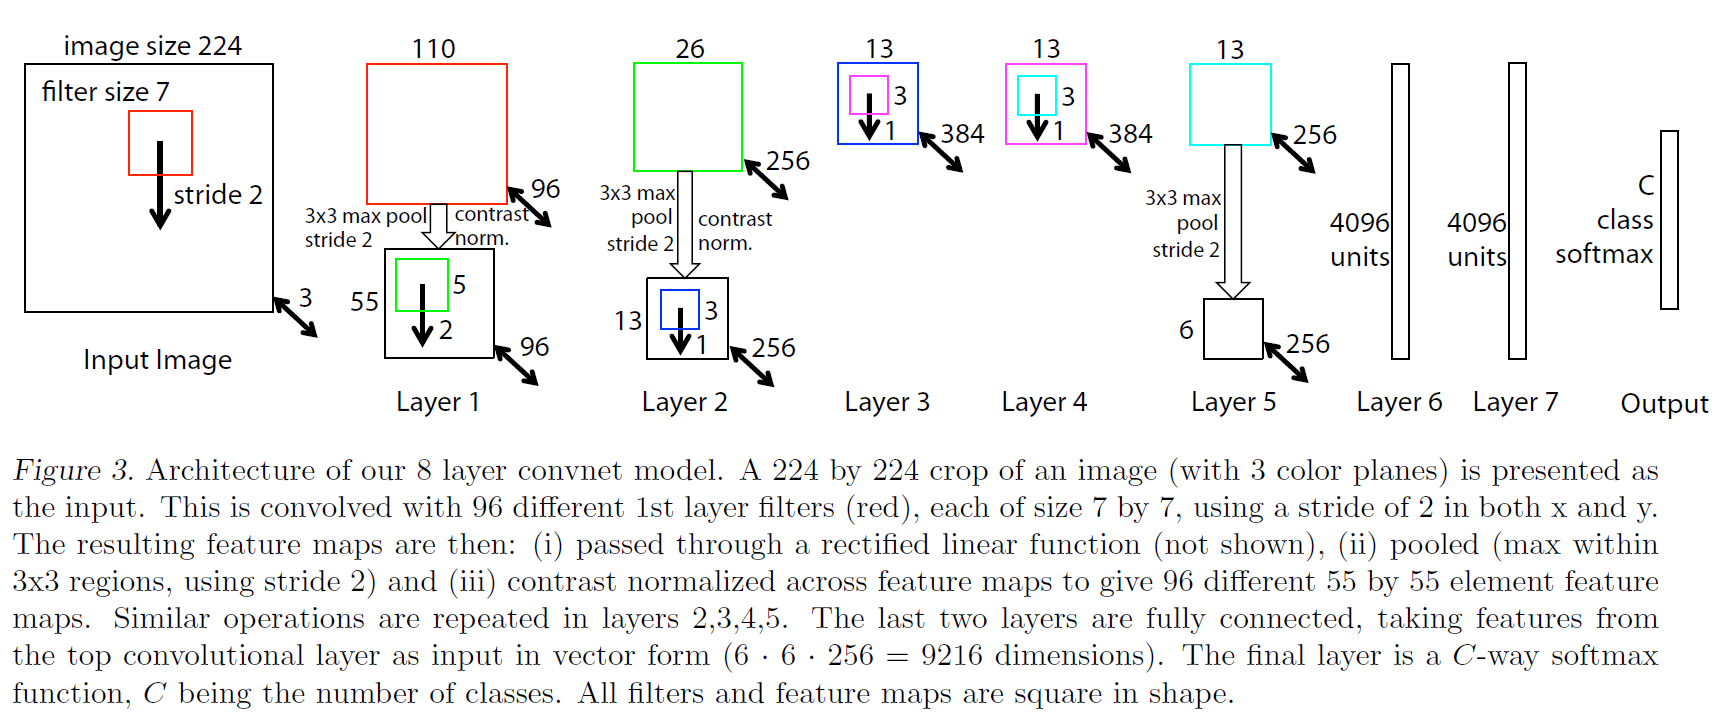
\includegraphics[scale=0.5]{figs/ZFNet_structure}
	\end{center}
	
\end{frame}

\begin{frame}
	\frametitle{Results in classification}
	\begin{center}
		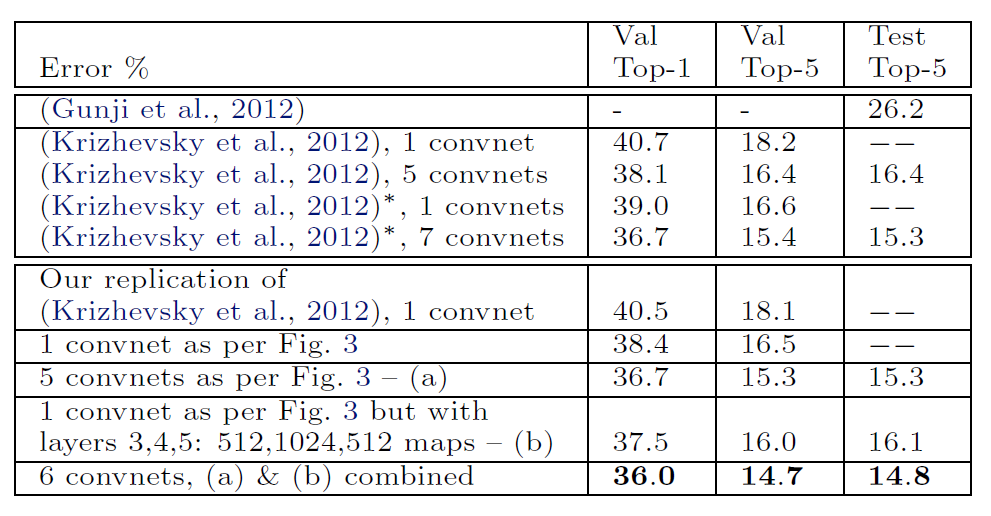
\includegraphics[scale=0.7]{figs/ZFNet_classif_results}
	\end{center}
\end{frame}

\begin{frame}[allowframebreaks]
	\frametitle{Occlusion}
	
	\begin{center}
		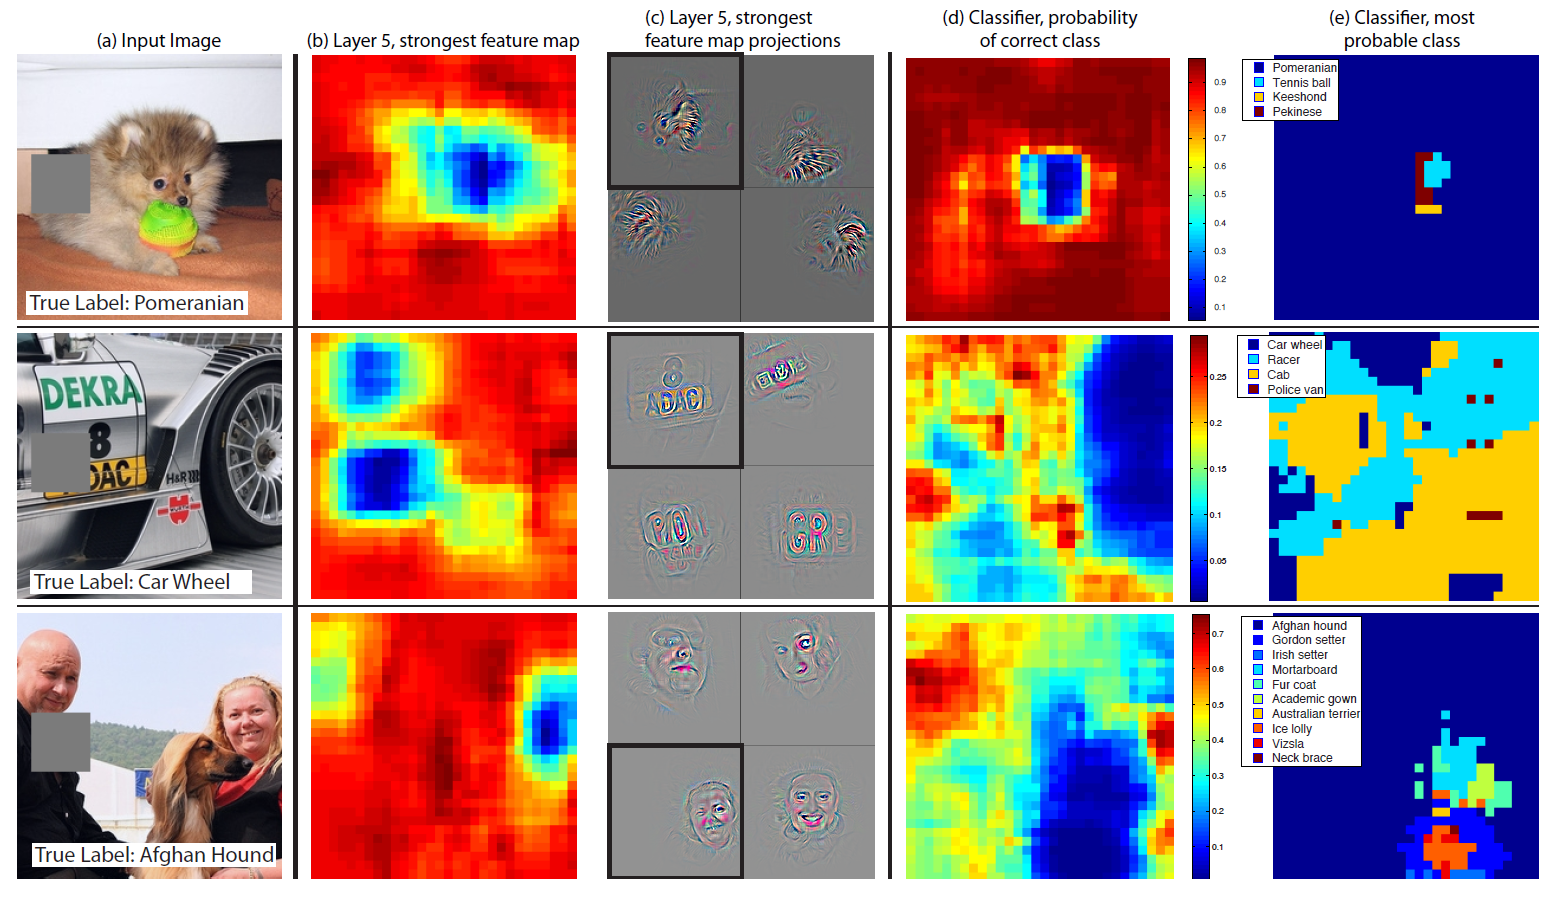
\includegraphics[scale=0.5]{figs/ZFNet_occlusion}
	\end{center}

\framebreak 

Three test examples where we systematically cover up different portions of the scene with a gray square (1st
column) and see how the top (layer 5) feature maps ((b) \& (c)) and classifier output ((d) \& (e)) changes. 

\medskip  


(b): for each
position of the gray scale, we record the total activation in one layer 5 feature map (the one with the strongest response
in the unoccluded image). 

\smallskip 

(c): a visualization of this feature map projected down into the input image (black square), along with visualizations of this map from other images. The first row example shows the strongest feature to be the
dog's face. When this is covered-up the activity in the feature map decreases (blue area in (b)). 

\smallskip 
(d): a map of correct
class probability, as a function of the position of the gray square. E.g. when the dog's face is obscured, the probability
for pomeranian drops significantly. 

\smallskip 
(e): the most probable label as a function of occluder position. 
%E.g. in the 1st row, for most locations it is pomeranian, but if the dog's face is obscured but not the ball, then it predicts tennis ball". In the 2nd example, text on the car is the strongest feature in layer 5, but the classifier is most sensitive to the wheel. The 3rd example contains multiple objects. The strongest feature in layer 5 picks out the faces, but the classifier is sensitive to the dog (blue region in (d)), since it uses multiple feature maps.
\end{frame}











\subsection{VGGNet (2014)}

\begin{frame}
	\frametitle{Tiny VGGnet}
	
		\citem{simonyan2014very}
		
		\bigskip 
		
	\begin{center}
		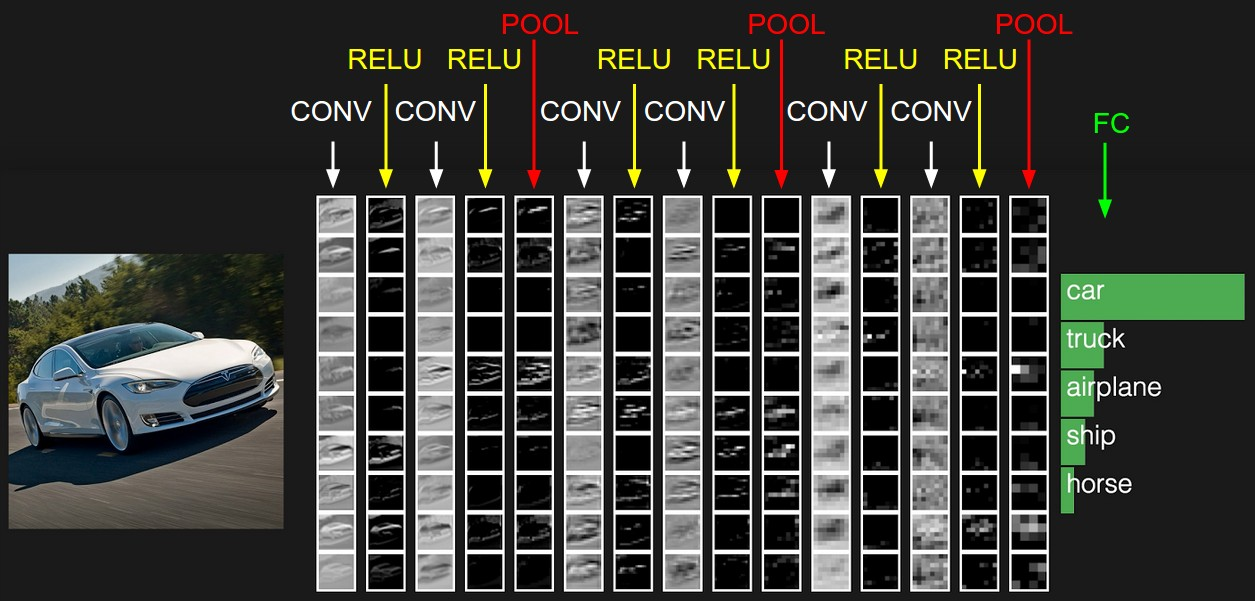
\includegraphics[scale=0.25]{figs/convnet}
	\end{center}
\end{frame}

\begin{frame}
	\frametitle{Network features}
	
	Convolutional layers:
	\begin{itemize}
		\item Small receptive field: $3 \times 3$ (smallest ones capable of capturing the notion of top/down, left/right!)
		\item Stride of $1$
		\item Spatial resolution is preserved after convolution
	\end{itemize} 
	
	\bigskip
	
	Max-pooling layers:
	\begin{itemize}
		\item $2 \times 2$ kernel
		\item Stride of $2$
	\end{itemize} 

	\bigskip
	
	All hidden layers make use of Rectified Linear Unit. 
	
	\bigskip
	
	Local Response Normalization layers do not improve performance. 
	 
\end{frame}

\begin{frame}
	\frametitle{Insightful remark...}
	
	\justifying 
	
	If you stack 3 convolutional layers with receptive fields $3 \times 3$, you obtain a convolutional layer with receptive fields $7\times 7$. What is the interest?
	
	\bigskip
	
	\begin{enumerate}
		\item Stack of $3$ convolutional layers of size $3 \times 3$: complexity of $3(3^2C^2) =27C^2$, where $C$ is the number of channels. 
		
		\medskip 
		
		\item One standard convolutional layer of size $7 \times 7$: complexity of $49C^2$. 
	\end{enumerate}
	
	\bigskip 
	
	In the first case, we cannot obtain every possible layer: the resulting object must  decompose as three consecutive convolutional layers. There are less possibilities hence less parameters. 
	
	 
	
\end{frame}



\begin{frame}
	\frametitle{VGGNet}
	
	\begin{center}
		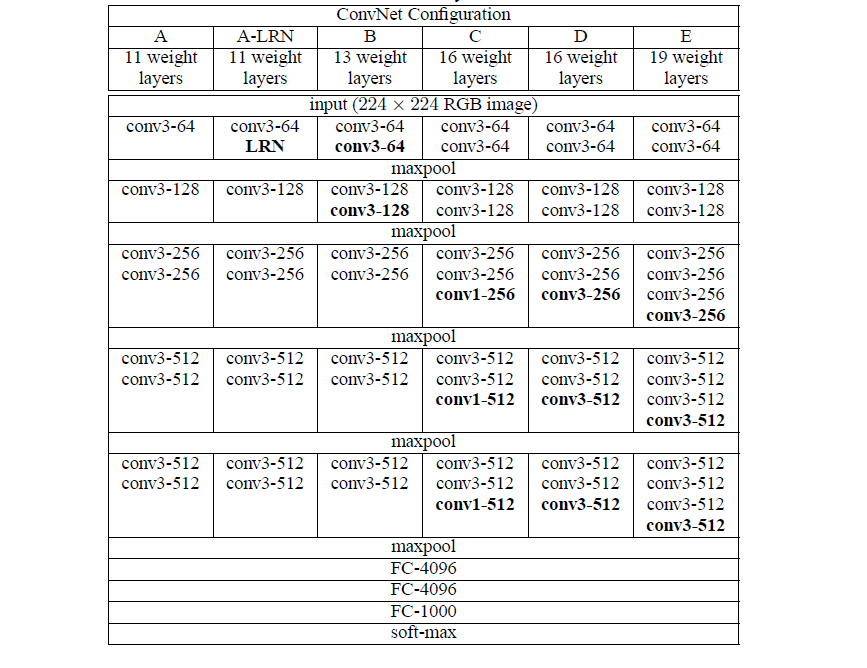
\includegraphics[scale=0.7]{figs/VGGNet_structure}
	\end{center}
	
	\begin{center}
		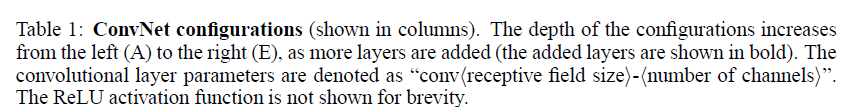
\includegraphics[scale=0.7]{figs/VGGNet_caption}
	\end{center}
\end{frame}






\begin{frame}
	\frametitle{Parameters}
	
	Initialization: 
	\begin{itemize}
		\item Network $A$: $\mathcal{N}(0, 0.01)$ for weights and $0$ for biases. 
		\item For other networks: first four conv layers and last three fully connected layers were initialized using network $A$ and the remaining layers were initialized randomly. 
	\end{itemize}
	
	
	
	
	\begin{block}{Stochastic gradient descent with momentum}
		\begin{align*}
			v^{(k+1)} & = 0.9 v^{(k)} - 0.0005 \eta \theta^{(k)} - \eta \frac{1}{B} \sum_{i \in \mathcal{B}} \nabla L_i (\theta^{(k)})\\
			\theta^{(k+1)} & = \theta^{(k)} + v^{(k+1)},
		\end{align*}	
		with batch size $B= 128$. 
	\end{block}
	
	
	
	Learning rate is the same for all layers with the following heuristic: 
	\begin{itemize}
		\item Initialization: $\eta = 0.01$
		\item Divide $\eta$ by $10$ when the validation error stop improving
		(this has been done three times).
		\item $74$ epochs.
	\end{itemize}
	
	\begin{itemize}
		\item $L_2$ penalty with constant $5.10^{-4}$
		\item Dropout regularization for the first two fully connected layers (probability of $0.5$)
	\end{itemize}
\end{frame}



\begin{frame}
	\frametitle{Results}
	
\begin{center}
	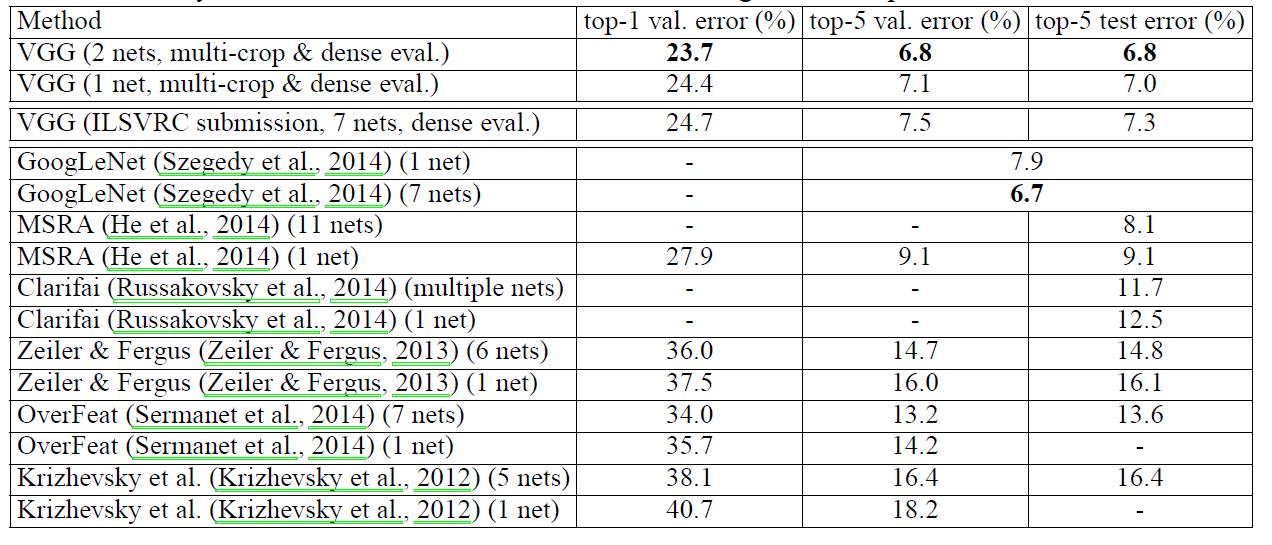
\includegraphics[scale=0.6]{figs/results_VGG}
\end{center}
	

	A downside of the VGGNet is that it is more expensive to evaluate and uses a lot more memory and parameters (140M). 
	
	Most of these parameters are in the first fully connected layer, and it was since found that these FC layers can be removed with no performance downgrade, significantly reducing the number of necessary parameters.
	
	%Dense evaluation: transform the fully connected layers into convolutional layers. Competitive compared to multi-crop (subsamples of images)
\end{frame}


\subsection{GoogLeNet (2014)}

\begin{frame}
	\frametitle{GoogLeNet}
	
	\citem{szegedy2015going}
	
	\bigskip
	
	Idea: increasing the depth and width of state-of-the-art convolutional neural networks while \blue{keeping the number of parameters small}:
	\begin{itemize}
		\item to be robust to overfitting
		
		\smallskip
		\item to be computationally appealing 
	\end{itemize}
	
	\bigskip
	
	Specifically, use of $1\times 1$ convolution layers to reduce the number of parameters + apply filters of different sizes $3 \times 3$, $5 \times 5$ or $3 \times 3$ max pooling (on each feature maps).

\bigskip 

All convolution layers use ReLU. 

\bigskip

Same spatial resolution for each feature map.

	
\end{frame}

\begin{frame}
	\frametitle{GoogLeNet - Inception module}
	
	Same spatial resolution for each feature map. 
	
	\smallskip
		
	Use of $1\times 1$ convolution layers to reduce the number of parameters then apply filters of different sizes $3 \times 3$, $5 \times 5$ or $3 \times 3$ max pooling (on each feature maps).
	
	

\begin{center}
	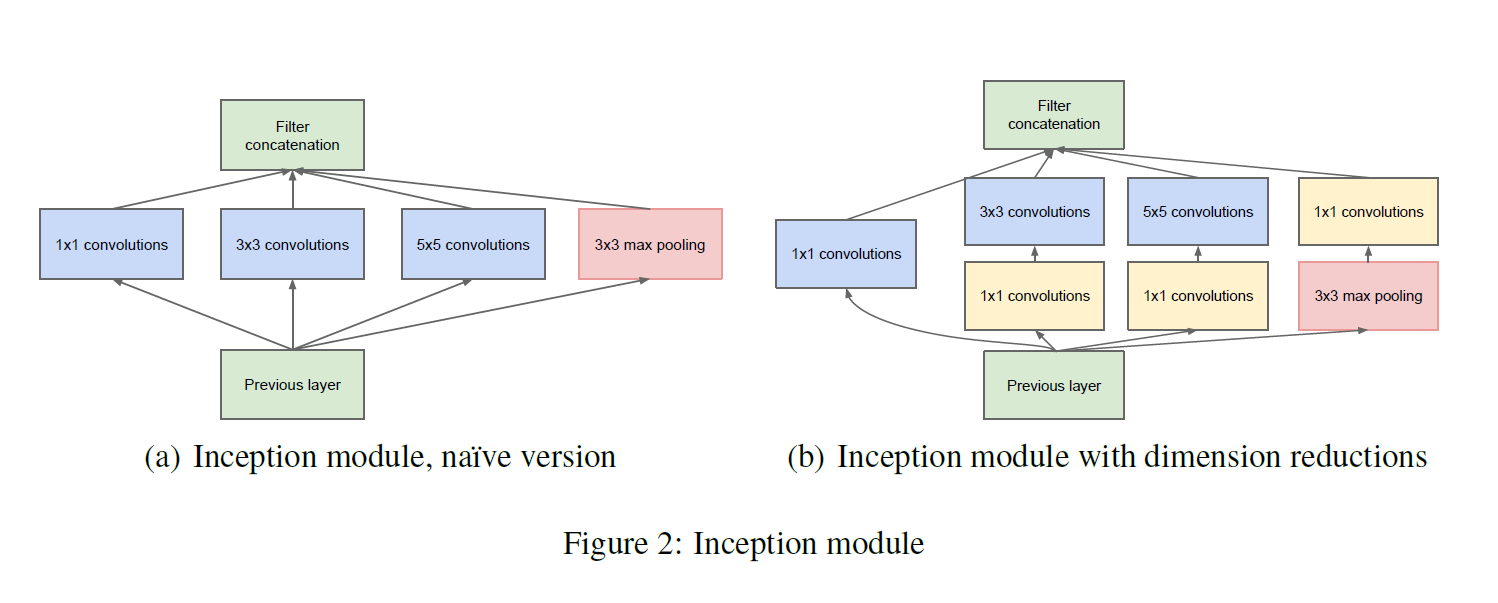
\includegraphics[scale=0.65]{figs/GoogLeNet_inception_module}
\end{center}
	
	
	
\end{frame}

\begin{frame}
	\frametitle{GoogLeNet - Inception module}
	
	\vspace{-0.8cm}
	
	\begin{center}
		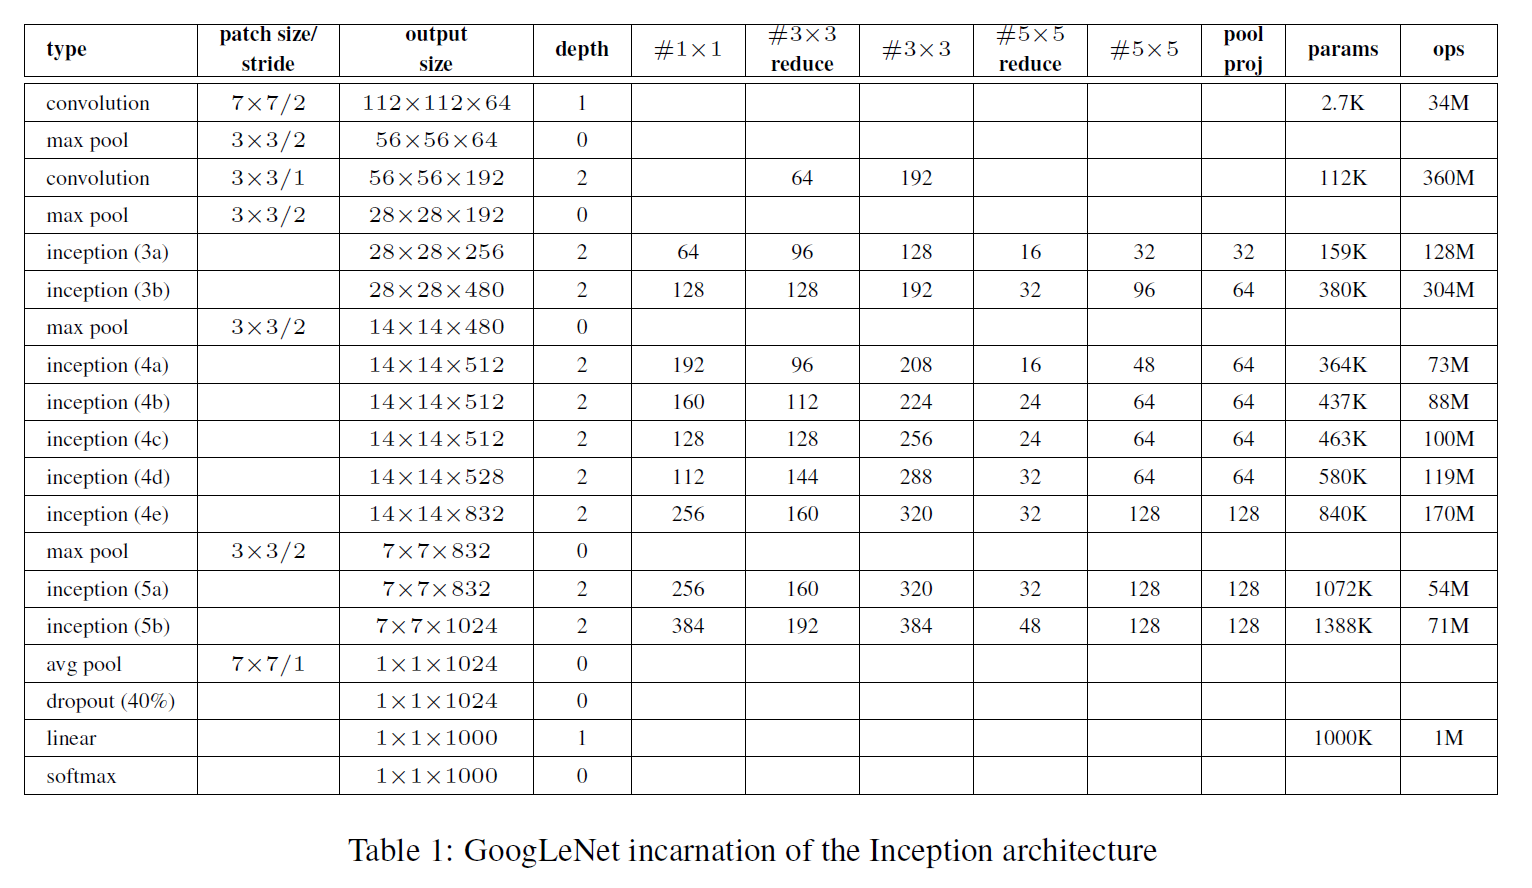
\includegraphics[scale=0.6]{figs/GoogLeNet_structure}
	\end{center}
	
	{\footnotesize ``3x3 reduce'' and ``5x5 reduce'' stands for the number of 1x1 filters in the reduction
	layer used before the 3x3 and 5x5 convolutions. One can see the number of 1x1 filters in the projection
	layer after the built-in max-pooling in the pool proj column.}
	
\end{frame}

\begin{frame}[allowframebreaks]
	\frametitle{Structure of GoogLeNet}
	
	\begin{center}
		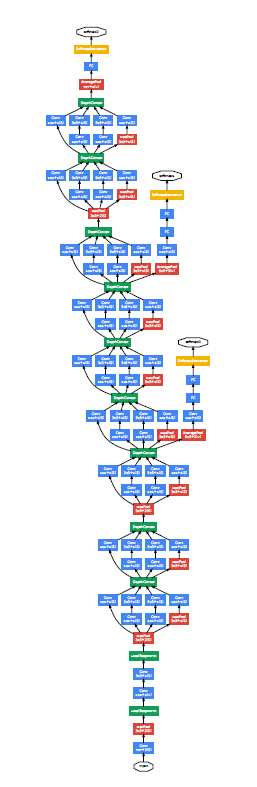
\includegraphics[scale=0.7]{figs/GoogLeNet_scheme}
	\end{center}
	
	\framebreak
	
	\frametitle{Structure of GoogLeNet}
	\begin{columns} % align columns
		
			\begin{column}{.2\textwidth}
			\begin{center}
				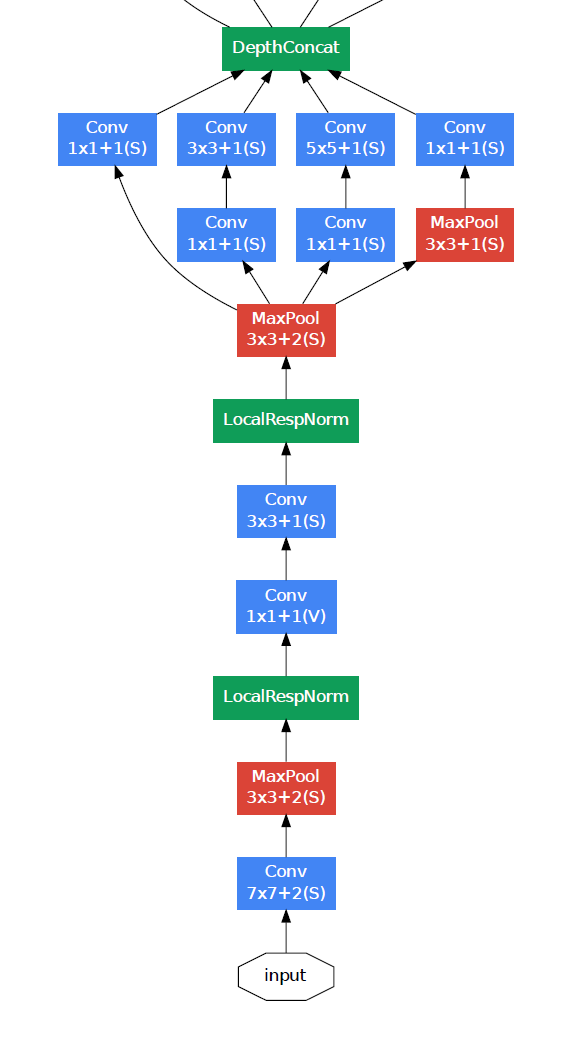
\includegraphics[scale=0.5]{figs/GoogleNet_scheme_2}
			\end{center}	
		\end{column}%
	
		\begin{column}{.4\textwidth}
			\begin{center}
				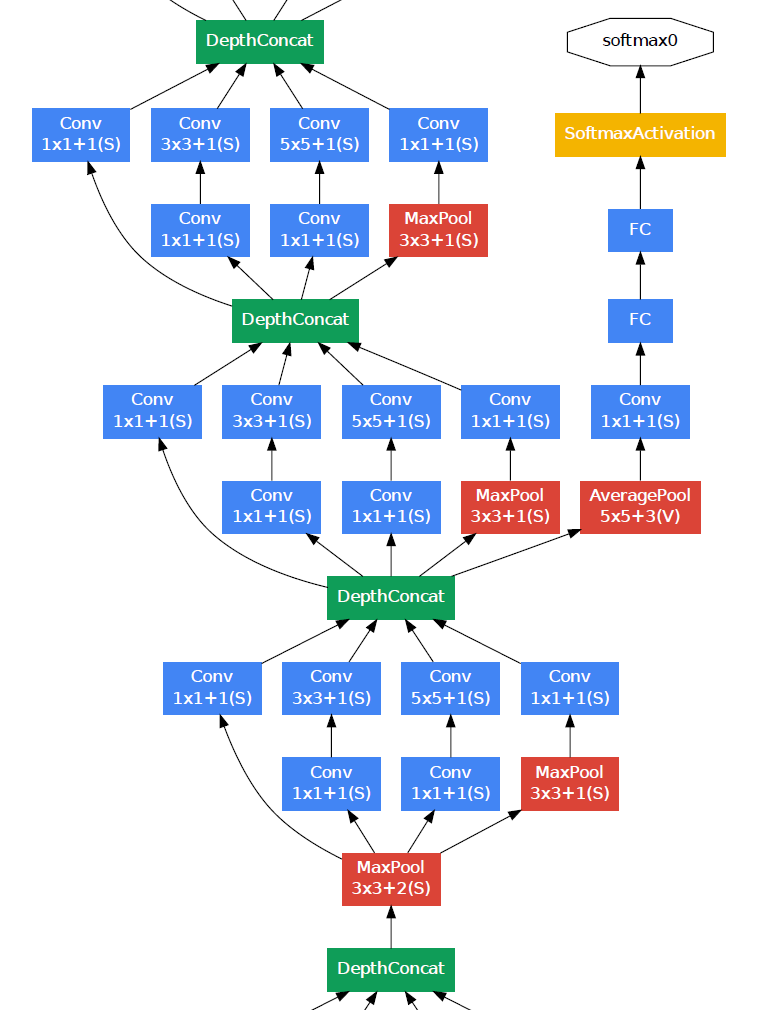
\includegraphics[scale=0.5]{figs/GoogleNet_scheme_1}
			\end{center}
		\end{column}
		
		
	
		
		\begin{column}{.4\textwidth}
		\begin{center}
			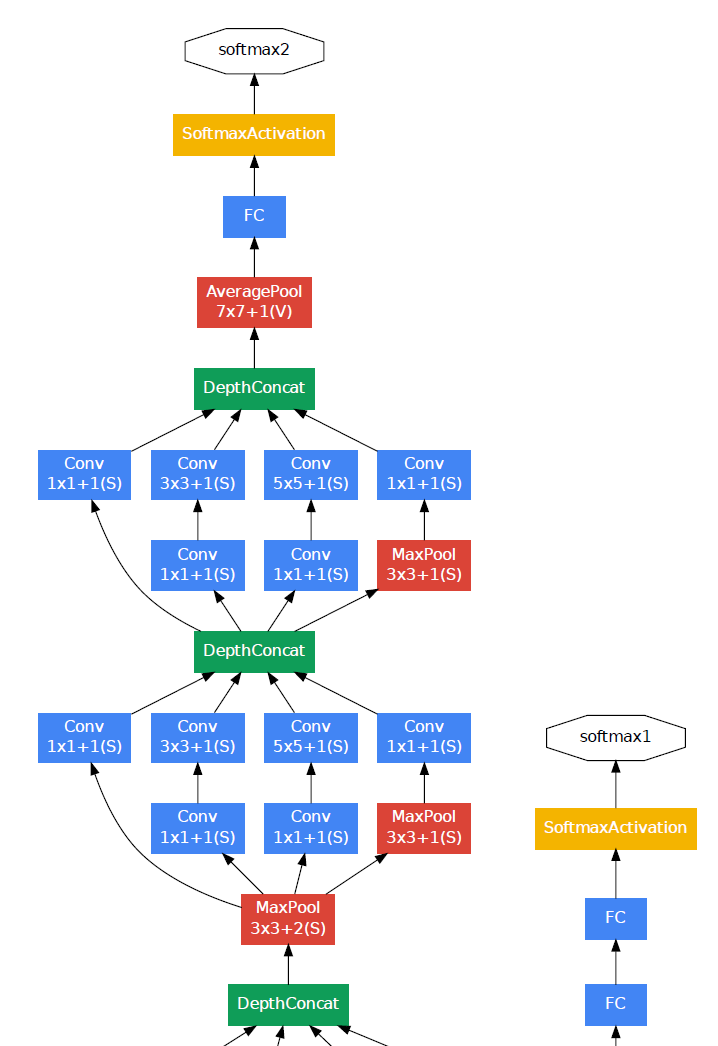
\includegraphics[scale=0.5]{figs/GoogleNet_scheme_3}
		\end{center}
		\end{column}%
	\end{columns}
	
	
	


	

\end{frame}

\begin{frame}
	\frametitle{Deep network - A concern}
	
	In order to backpropagate gradient, the authors add some auxiliary classifiers connected to intermediate layers.
	
	\smallskip 
	During training the loss of auxiliary classifiers is weighted by $0.3$ and added to the total loss of the network. Auxiliary networks are removed at inference time. 
	
	\bigskip 
	
	Auxiliary network put after $(4a)$ and $(4d)$: 
	\begin{itemize}
		\item Average pooling layer $5\times 5$, stride of $3$
		\item A $1 \times 1$ convolution with $128$ filters, with ReLU.
		\item A fully connected layer with $1024$ neurons and ReLU
		\item A dropout layer with a dropout ratio of $70\%$.
		\item A linear layer with softmax loss, predicting the same $1000$ classes as the main classifier.
	\end{itemize}
	
\end{frame}




\begin{frame}
	\frametitle{Parameters}
	
	Initialization: 
	\begin{itemize}
		\item Each random unit is connected to $15$ randomly chosen units in the previous layer
		\item Corresponding weights are drawn from $\mathcal{N}(0,1)$ and biases are set to $0$. 
	\end{itemize}
	\citem{martens2010deep}
	
	
	
	\begin{block}{Stochastic gradient descent with momentum}
		\begin{align*}
			v^{(k+1)} & = \mu  v^{(k)} - \eta \frac{1}{B} \sum_{i \in \mathcal{B}} \nabla \ell_i (\theta^{(k)} + \mu  v^{(k)})\\
			\theta^{(k+1)} & = \theta^{(k)} + v^{(k+1)},
		\end{align*}	
		with batch size $B= 200$, where
		$$
		\mu^{(k)} = \min (1 - 2^{-1 - \log2(\lfloor t/250 \rfloor +1)}, \mu_{max}),
		$$
		where $\mu_{max} \in \{0, 0.9, 0.99, 0.995, 0.999\}$.
	\end{block}
	
	
	
	Learning rate is the same for all layers with the following heuristic: 
	\begin{itemize}
		\item Initialization: $\eta = 0.01$
		\item Multiply $\eta$ by $0.96$ every $8$ epochs.
		\item $750000$ parameter updates = $125$ epochs.
	\end{itemize}
	





\end{frame}




\begin{frame}
	\frametitle{Results}
	
		\vspace{-0.4cm}
		
		\begin{itemize}
		\item Polyak averaging is used to create the final model at inference time. 
		\item $7$ different versions of GoogleNet were trained and aggregated to make predictions. 
	\end{itemize}


	\begin{center}
		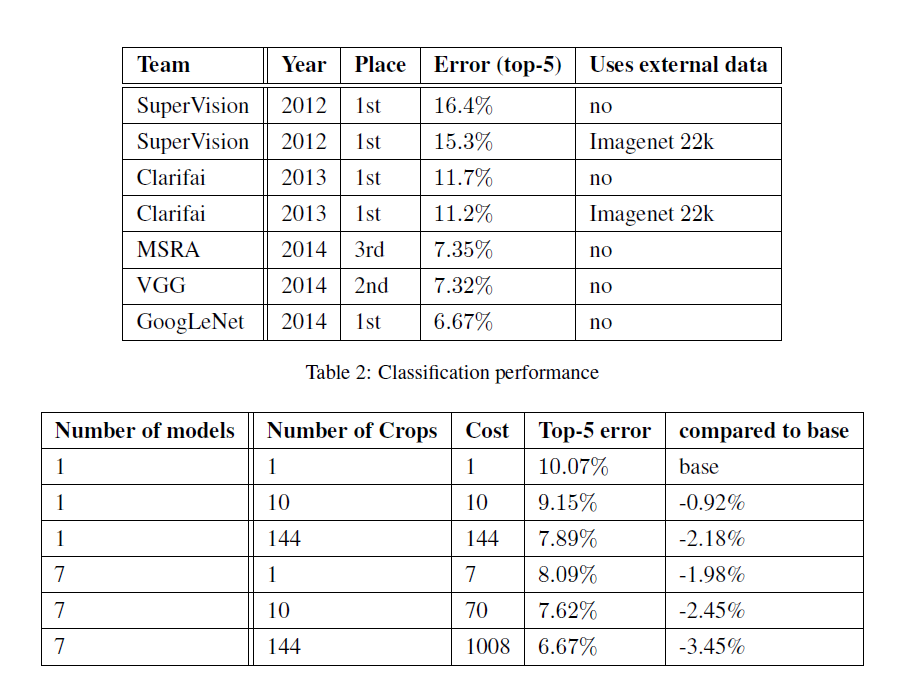
\includegraphics[scale=0.7]{figs/GoogleNet_results}
	\end{center}	



		{\small Main contribution: development of an Inception Module that dramatically reduced the number of parameters in the network (4M, compared to AlexNet with 60M). }
		
\end{frame}


\subsection{ResNet (2016)}

\begin{frame}
	\frametitle{ResNet (2016)}
	
	\citem{he2016deep}
		
	\bigskip 	
		
	\blue{Statement}: Optimization can be hard for some deep networks.
	
	\bigskip 
	
	\blue{Solution}: Ease optimization by adding simple paths in the network
	
	\bigskip 
	
	\begin{center}
		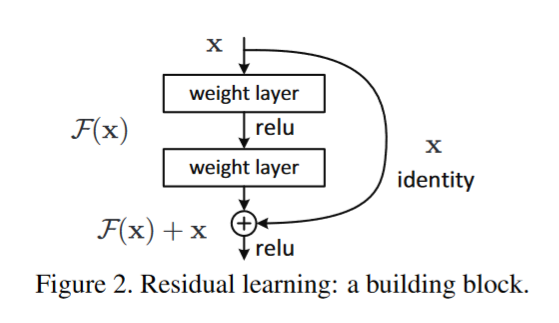
\includegraphics[scale=0.7]{figs/ResNet_IdentityBlock}
	\end{center}
	
	\medskip 
	$\rightarrow$ No extra parameters, no additional computational complexity
\end{frame}

\begin{frame}
	\frametitle{Literature on shortcut connections}
	
	Early practice for training multi layers perceptrons was to add a linear layer between the inputs and the outputs
	
	\citem{ripley2007pattern}
	
	\bigskip 
	
	Few intermediate classifiers can also be added in intermediary levels in order to ease the optimization: 
	\begin{itemize}
		\item 	\citem{szegedy2015going}
		\item 	\citem{lee2015deeply}
	\end{itemize}

	\bigskip 

	Highway networks have shortcut connections with gating functions.
	Here, gates are data dependent and have parameters. 
	
	\begin{itemize}
		\item \citem{srivastava2015highway}
		\item \citem{srivastava2015training}
	\end{itemize}

\end{frame}

\begin{frame}
	\frametitle{General Idea}
	
	Inspired from VGG nets:
	
	\smallskip 
	\begin{itemize}
		\item For the same output feature map size, the layers have the same numbers of filters
		\item If the feature map size is halved, then the number of filters is doubled to preserve the time complexity per layer
	\end{itemize}
$$
\textbf{y} = f(\textbf{x}, \textbf{W}_i) \blue{+ \textbf{x}},
$$

\smallskip 
where $\textbf{x}$ and $\textbf{y}$ are respectively the input and the output of a (stack of) layer(s), $\textbf{W}_i$ are the weights of this/these layer(s) and $f(\textbf{x}, \textbf{W}_i)$ the output of this/these layer(s).

\bigskip 

If dimensions do not match between $\textbf{x}$ and $\textbf{y}$, there are two solutions: 
\begin{itemize}
	\item identity mapping is coupled with extra zero entries padded for increasing dimensions
	\item Projection shortcut is used to match dimensions via $1 \times 1$ convolution filters
	$$
	\textbf{y} = f(\textbf{x}, \textbf{W}_i) + W_s \textbf{x},
	$$
	where $W_s$ is a projection.
\end{itemize}

\end{frame}


\begin{frame}[allowframebreaks]
	\frametitle{Structure of ResNet}
	
	\begin{center}
		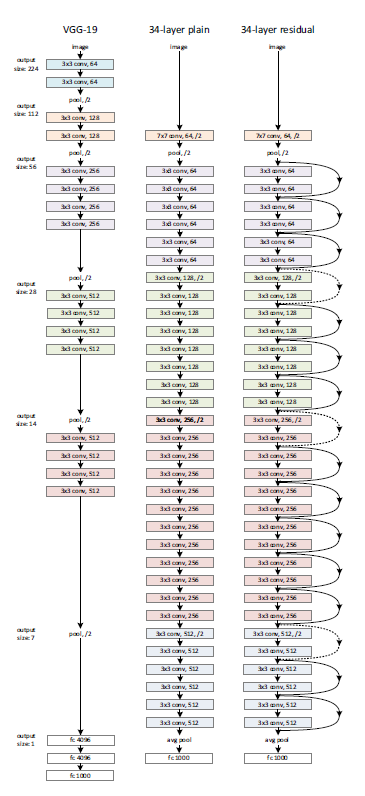
\includegraphics[scale=0.5]{figs/ResNet_structure}
	\end{center}

\framebreak

\frametitle{Structure of ResNet}
\begin{columns} % align columns
	
	
	\begin{column}{.5\textwidth}
		\begin{center}
			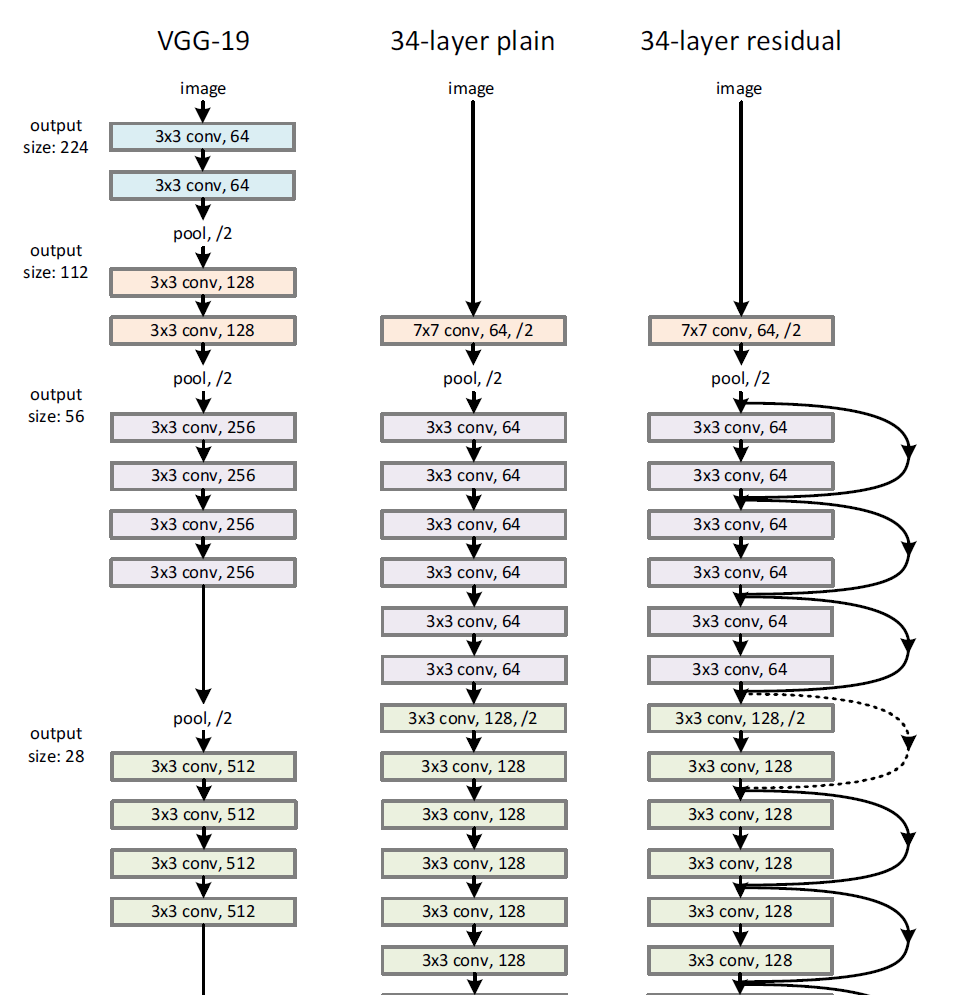
\includegraphics[scale=0.5]{figs/ResNet_zoom1}
		\end{center}
	\end{column}
	
	
	
	
	\begin{column}{.5\textwidth}
		\begin{center}
			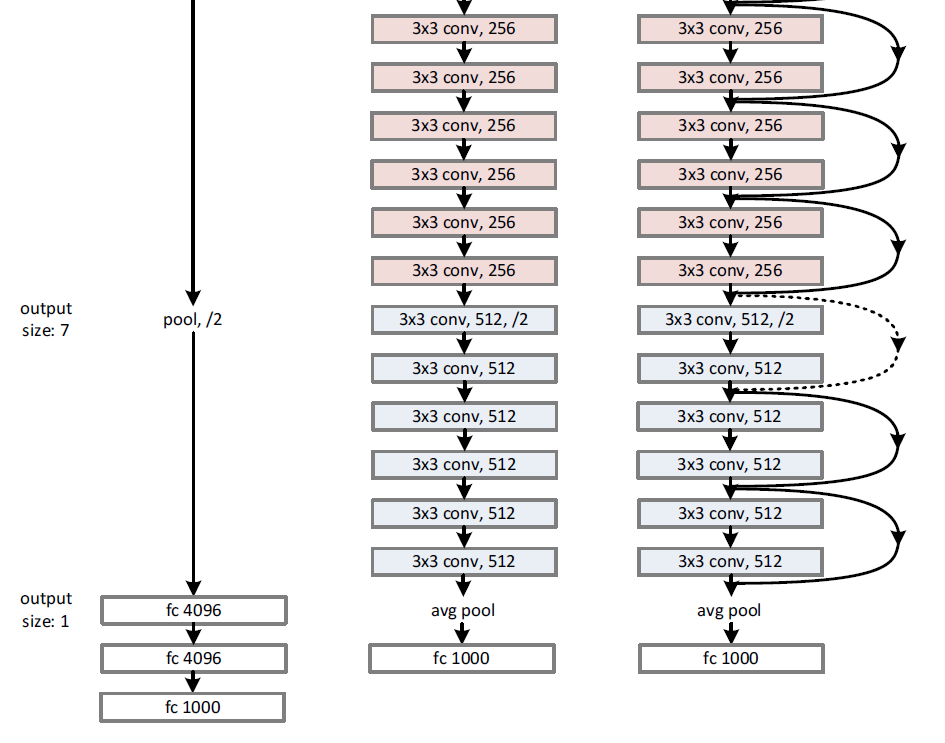
\includegraphics[scale=0.5]{figs/ResNet_zoom2}
		\end{center}
	\end{column}%
\end{columns}



\end{frame}




\begin{frame}
	\frametitle{Parameters}
	
Initialization, as in \cite{he2015delving}: weights are drawn from $\mathcal{N}(0, 2/n_L)$ ($n_L$ is the number of neurons in the previous layer); biases are set to $0$. 

	
	\begin{block}{Stochastic gradient descent with momentum}
		\begin{align*}
			v^{(k+1)} & = 0.9 v^{(k)} - 0.0001 \eta \theta^{(k)} - \eta \frac{1}{B} \sum_{i \in \mathcal{B}} \nabla L_i (\theta^{(k)})\\
			\theta^{(k+1)} & = \theta^{(k)} + v^{(k+1)},
		\end{align*}	
		with batch size $B= 256$. 
	\end{block}
	
	
	
	Learning rate is the same for all layers with the following heuristic: 
	\begin{itemize}
		\item Initialization: $\eta = 0.1$
		\item Divide $\eta$ by $10$ when the validation error stop improving
		(this has been done three times).
		\item $120$ epochs.
	\end{itemize}
	
	Miscellaneous: 
	\begin{itemize}
		\item Batch normalization after each convolution and before activation
		\item No dropout
	\end{itemize}
\end{frame}


\begin{frame}
	\frametitle{Results}
	

	\begin{center}
		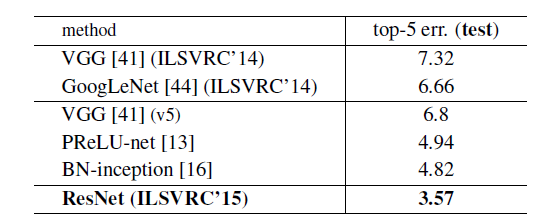
\includegraphics[scale=1]{figs/ResNet_results}
	\end{center}

	\bigskip 
	
	\begin{itemize}
		\item Winner of ILSVRC 2015
		\item Special skip connections and heavy use of batch normalization
		\item No fully connected layers at the end of the network. 
	\end{itemize}
	


\end{frame}




\subsection{DenseNet (2017)}

\begin{frame}
\frametitle{DenseNet}

\citem{huang2017densely}

\bigskip

\begin{center}
	\begin{figure}
		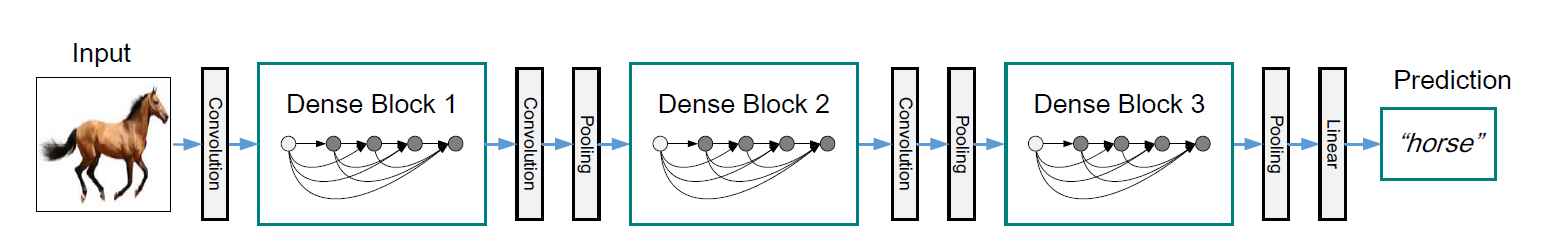
\includegraphics[scale=0.6]{figs/densenet_scheme2}
		\caption{A deep DenseNet with three dense blocks. The layers between two adjacent blocks are referred to as transition layers and change
		feature-map sizes via convolution and pooling}
	\end{figure}
\end{center}

\end{frame}

\begin{frame}
	\frametitle{DenseNet}

\begin{center}
	\begin{figure}
		\includegraphics[scale=0.7]{figs/densenet_scheme}
		\caption{A 5-layer dense block with a growth rate of $k = 4$.
			Each layer takes all preceding feature-maps as input.}
	\end{figure}

\end{center}
\end{frame}

\begin{frame}[allowframebreaks]
	\frametitle{Ingredients}
	
	
	
	Let $\textbf{x}_{\ell}$ be the input of the $\ell$th layer. Usually, 
	$$
	\textbf{x}_{\ell} = f_{\ell}(\textbf{x}_{\ell-1}).
	$$

\bigskip 

\textbf{Dense Block}. Inside a dense block,
	$$
	\textbf{x}_{\ell} = f_{\ell}(\textbf{x}_{0}, \hdots, \textbf{x}_{\ell-1}).
	$$
	
	The functions $f_{\ell}$ are composed of three consecutive operations: 
	\begin{enumerate}
		\item First, a batch normalization
		\item Then, activation function ReLU
		\item Finally, $3 \times 3$ convolutional layer (feature map sizes are kept fixed)
	\end{enumerate}

\bigskip 

\textbf{Between dense blocks}.
	\begin{enumerate}
		\item Batch normalization
		\item $1 \times 1$ convolution
		\item $2 \times 2$ average pooling
	\end{enumerate}

\framebreak 

\textbf{Growth rate $k$}

If each function $f_{\ell}$ produces $k$ feature maps, the inputs of the $\ell$th layer has $k_0 + k(\ell-1)$ channels. Narrow layers (typically $k=12$) give good results. 

$\rightarrow$ Indeed, each layer has access to each previous layer and thus to the ``collective knowledge'' of the network. 

\bigskip 

\textbf{Bottleneck layer} - DenseNet-B 

A way to improve computational efficiency is to introduce $1 \times 1$ convolutional layers in the form 
\begin{center}
	BN - ReLU - Conv ($1 \times 1$) - BN - ReLU - Conv ($3 \times 3$)
\end{center}
Conv  $1 \times 1$ typically produces $4k$ feature maps. 

\bigskip 

\textbf{Compression layer} - DenseNet-C

Throw away a fraction $\theta \in [0,1]$ (typically $\theta=0.5$) of feature maps at transition layers.
\end{frame}










\begin{frame}
	\frametitle{Architecture}
	
	\begin{center}
		\includegraphics[scale=0.65]{figs/densenet_architecture}
	\end{center}
\end{frame}




\begin{frame}
\frametitle{Parameters}

Initialization, as in \cite{he2015delving}: weights are drawn from $\mathcal{N}(0, 2/n_L)$ ($n_L$ is the number of neurons in the previous layer); biases are set to $0$. 


\begin{block}{Stochastic gradient descent with momentum}
	\begin{align*}
	v^{(k+1)} & = 0.9 v^{(k)} - 0.0001 \eta \theta^{(k)} - \eta \frac{1}{B} \sum_{i \in \mathcal{B}} \nabla L_i (\theta^{(k)})\\
	\theta^{(k+1)} & = \theta^{(k)} + v^{(k+1)},
	\end{align*}	
	with batch size $B= 256$. 
\end{block}



Learning rate is the same for all layers with the following heuristic: 
\begin{itemize}
	\item Initialization: $\eta = 0.1$
	\item Divide $\eta$ by $10$ at epoch $30$ and $60$.
	\item $90$ epochs.
\end{itemize}

Miscellaneous: 
\begin{itemize}
	\item Batch normalization after each convolution and before activation
	\item No dropout
\end{itemize}
\end{frame}

\begin{frame}
\frametitle{DenseNet Results }

\vspace{-0.4cm}
\begin{center}
	\includegraphics[scale=0.6]{figs/DenseNet_results}
\end{center}
\end{frame}

%
%\section{Mathematics behind CNN}
%
%\subsection*{Where is convolution?}
%
%\subsection*{Backpropagation}



















\section{Applications}

\begin{frame}
	\frametitle{Applications}
	This section is based on \citem{gu2015recent}.
	
	\bigskip 
	
	More applications domain and more references are presented in this paper. 
	
	\bigskip
	
	\medskip 
	
	\begin{center}
		\includegraphics[scale=0.6]{figs/cat_detector}
	\end{center}


\end{frame}
\subsection{Image classification}



\begin{frame}
\frametitle{Image classification - Hierarchy of classifiers}





\citem{xiao2014error}

\smallskip
$\rightarrow$ They propose a training method that grows a network not only incrementally but also hierarchically. In their method, classes are grouped according to similarities and are self- organized into different levels. 

\bigskip 


\citem{yan2015hd}

\smallskip
$\rightarrow$ They introduce a hierarchical deep CNNs (HD-CNNs) by embedding deep CNNs into a category hierarchy. They decompose the classification task into two steps. The coarse category CNN classifier is first used to separate easy classes from each other, and then those more challenging classes are routed downstream to fine category classifiers for further prediction. This architecture follows the coarse-to-fine classification paradigm and can achieve lower error at the cost of an affordable increase of complexity.



\end{frame}



\begin{frame}[allowframebreaks]
\frametitle{Image classification - CNN Tree}

\cite{wang2018learning} build a tree of CNN to learn fine-grained features for subcategory recognition. 

\begin{center}
	\includegraphics[scale=0.8]{figs/CNNTree_scheme.png}
\end{center}

\framebreak

\begin{figure}
\begin{center}
	\includegraphics[scale=0.8]{figs/CNNTree_confusion_matrix_softmax}
\end{center}
\caption{Confusion set outputs by AlexNet softmax prediction on validation set of ILSVRC 2015.}
\end{figure}




\framebreak


\begin{center}
	\includegraphics[scale=0.7]{figs/CNNTree_result1.PNG}
\end{center}


\begin{center}
	\includegraphics[scale=0.7]{figs/CNNTree_results2.PNG}
\end{center}

\framebreak

\begin{figure}
	
\begin{center}
	\includegraphics[scale=0.55]{figs/CNNTree_imageclassification}
\end{center}
\caption{Top label is given by basic AlexNet CNN while bottom one is given by CNNTree (green color corresponds to a correct prediction)}
\end{figure}

\end{frame}


\subsection{Pose, action detection}


\begin{frame}[allowframebreaks]
\frametitle{Pose estimation - Deeppose}

 \citem{toshev2014deeppose} 

\bigskip

DeepPose  is the first application of CNNs to human pose estimation problem. It captures the full context of each body joint by taking the whole image as the input.

\bigskip

Previous works: 
\begin{itemize}
	\item Limited expressiveness – the use of local detectors, which
	reason in many cases about a single part
	\item Modeling only a small subset of all interactions
	between body parts.
\end{itemize}

\framebreak

Structure: 
\begin{itemize}
	\item Normalizing images
	\item Regression problem, i.e., prediction of $k$ joints
	$$
	\textrm{Image} \mapsto \textbf{y} \in \R^{2k}.
	$$
	\item Use a cascade of $7$ layers, each one taking a zoom of the previous image as input (refinement of the prediction at each stage).
\end{itemize}



\begin{center}
	\includegraphics[scale=0.6]{figs/Deeppose}
\end{center}

\framebreak

\begin{center}
	\includegraphics[scale=0.6]{figs/Deeppose_results1}
\end{center}

\framebreak

\begin{center}
	\includegraphics[scale=0.5]{figs/Deeppose_results2}
\end{center}





\end{frame}


\begin{frame}
\frametitle{Action recognition - images}


\blue{Action recognition} aims at classifying human activities based on their visual appearance and motion dynamics.

\bigskip 

In \cite{simonyan2014very} (VGG),they use the outputs of the penultimate layer of a pre-trained CNN to represent full images of actions as well as the human bounding boxes inside them, and achieve a high level of performance in action classification.

\bigskip 

 \cite{gkioxari2015actions} add a part detection to this framework. Their part detector is a CNN based extension to the original Poselet \cite{pishchulin2013poselet} method.

\end{frame}

\begin{frame}[allowframebreaks]
	\frametitle{Action recognition}
	
	\citem{gkioxari2015actions}
	
	\bigskip
	
	\begin{center}
		\includegraphics[scale=0.6]{figs/action_recognition_structure}
	\end{center}

\bigskip 

Given an R-CNN person detection (red box), they detect parts using a
novel, deep version of poselets. The detected whole-person and part bounding boxes are input into a fine-grained classification engine to produce predictions for actions and attributes.
	
	\framebreak
	
	\begin{center}
		\includegraphics[scale=0.6]{figs/results_picture_action_detection}
	\end{center}
	
\end{frame}
\subsection{Object detection}

\begin{frame}[allowframebreaks]
	\frametitle{Object detection - Exhaustive search vs segmentation}
	
	Segmentation: aims for
	a unique partitioning of the image through a generic algorithm,
	where there is one part for all object silhouettes in the image.
	
	\medskip 
	
\begin{columns} % align columns
		
		\begin{column}{.5\textwidth}
			\begin{center}
				\includegraphics[scale=0.6]{figs/selectivesearch_pictures}
			\end{center}
		\end{column}%
		

		
		\begin{column}{.4\textwidth}
		High variety of reasons that an image region forms an object: 
		
		
		
		\end{column}%
	\end{columns}
	
\medskip

	
\framebreak

Segmentation: aims for
a unique partitioning of the image through a generic algorithm,
where there is one part for all object silhouettes in the image.

\medskip 

\begin{columns} % align columns
	
	\begin{column}{.5\textwidth}
		\begin{center}
			\includegraphics[scale=0.6]{figs/selectivesearch_pictures}
		\end{center}
	\end{column}%
	
	
	
	\begin{column}{.4\textwidth}
		High variety of reasons that an image region forms an object: 
		
		\begin{itemize}
			\item[(b)] the cats can be distinguished by colour, not
			texture. 
			
			\item[(c)] the chameleon can be distinguished from the surrounding
			leaves by texture, not colour.
			
			\item[(d)]  the wheels can be part
			of the car because they are enclosed, not because they are similar
			in texture or colour. 
			
			\item[(a)] many different scales needed
		\end{itemize} 
		
	\end{column}%
\end{columns}

\medskip

$\rightarrow$ Necessity to use a variety of diverse strategies.


	
	\framebreak
	
	\blue{Alternative approach:} do localisation through the identification of an object.
	
	\bigskip
	
	\blue{Exhaustive search:} With an appearance model learned
	from examples, an exhaustive search is performed where every location
	within the image is examined as to not miss any potential
	object location.
	
	\medskip 
	
		
	Searching every possible location is computationally infeasible.

\medskip

$\rightarrow$ restrictions
	need to be imposed: the classifier is simplified and the appearance
	model needs to be fast.
	
		\bigskip
		
	\blue{Selective search:} data-driven selective search using bottom up grouping.
	
	\framebreak
	
	Bottom-up grouping generates hierarchical nested partitioning of the input image. 
	
	\citem{comaniciu2002mean, felzenszwalb2004efficient}
	
	\begin{center}
	\includegraphics[scale=0.4]{figs/selective_search_partitions.PNG}
	\end{center}

\framebreak 

Generic algorithm:
\begin{itemize}
	\item They first use \cite{felzenszwalb2004efficient} 
	to create initial regions. This method is the fastest, publicly
	available algorithm that yields high quality starting locations.
	
	\item Then they use a greedy algorithm to iteratively
	group regions together	
	\begin{itemize}
		\item First the similarities between all
		neighbouring regions are calculated. 
		\item The two most similar regions
		are grouped together, and new similarities are calculated between
		the resulting region and its neighbours. 
		\item The process of grouping
		the most similar regions is repeated until the whole image becomes
		a single region.
	\end{itemize}
\end{itemize}

Variety of partitionings:
\begin{itemize}
	\item Different variant of input images
	\item Similarities based on color, texture, size, shared pixels
\end{itemize}

\begin{center}
	\includegraphics[scale=0.6]{figs/selective_search_invariance_channel}
\end{center}

\framebreak


\begin{center}
	\includegraphics[scale=0.4]{figs/pipeline_selective_search}
\end{center}



\end{frame}


\begin{frame}
	\frametitle{Object detection - naive approach}
	
	
	Generally, the difficulties mainly lie in how to accurately and efficiently localize objects in images or video frames.
	
	\bigskip
	
	In some early works by \cite{vaillant1994original, nowlan1995convolutional, girshick2015deformable}, they use the sliding window based approaches to densely evaluate the CNN classifier on windows sampled at each location and scale. Since there are usually hundreds of thousands of candidate windows in a image, these methods suffer from highly computational cost, which makes them unsuitable to be applied on the large-scale dataset
	
	\bigskip
	
	More references on object proposal based methods: 

\smallskip 

 \citem{nguyen2016human}
 
 \citem{endres2014category}
 
 \citem{gomez2017textproposals}
	
\end{frame}

\begin{frame}[allowframebreaks]
	\frametitle{Object detection - R-CNN - Regions with CNN features}
	
	
	
	One of the most famous object proposal based CNN detector is Region-based CNN (R-CNN) by \cite{girshick2014rich}, aiming at 
	\begin{itemize}
		\item localizing objects with  a  deep  network
		\item training  a  high-capacity  model with only a small quantity of annotated detection data
	\end{itemize} 


	
\begin{columns} % align columns
	
	\begin{column}{.5\textwidth}
		\begin{center}
		\includegraphics[scale=0.6]{figs/RCNN_structure}
	\end{center}
	\end{column}%
	
	
	
	\begin{column}{.4\textwidth}
	\begin{enumerate}
		\item Generating category-independent region proposals via selective search.
		
		\item Training large CNN that extracts a fixed-length feature vector from each region (Supervised pre-training  on the large auxiliary dataset ILSVRC, followed by domainspecific   fine-tuning on the small dataset PASCAL).
		\item Learning a set of class-
		specific linear SVMs. 
	\end{enumerate}
	\end{column}%
\end{columns}

\framebreak 

\begin{center}
	\includegraphics[scale=0.6]{figs/mAP_RCNN}
\end{center}
However, computational cost is high since the time-consuming CNN feature extractor will be performed for each region separately.


\framebreak



\begin{center}
	\includegraphics[scale=0.5]{figs/RCNN_bad_classification}
\end{center}

\begin{center}
	\includegraphics[scale=0.6]{figs/RCNN_right_classification}
\end{center}

\end{frame}


\begin{frame}
	\frametitle{Object detection - improving R-CNN}
	
	\citem{he2014spatial}
	
	\blue{Spatial Pyramid Pooling} network (SPP net) is a pyramid-based version of R-CNN, which introduces an SPP layer to relax the constraint that input images must have a fixed size. Unlike R-CNN, SPP net extracts the feature maps from the entire image only once, and then applies spatial pyramid pooling on each candidate window to get a fixed-length representation. 
	
\textbf{Drawback:} multi-stage pipeline $\Rightarrow$ CNN feature extractor and SVM classifier are impossible to train jointly.
	
	\medskip 
	
	\citem{ren2015faster}
	
	\blue{Fast RCNN} improves SPP net by using an end-to-end training method. All network layers can be updated during fine-tuning, which simplifies the learning process and improves detection accuracy. 
	
	\medskip
	
	\citem{yoo2015attentionnet} 
	
	They treat the object detection problem as an iterative classification problem. It predicts an accurate object boundary box by aggregating quantized weak directions from their detection network.
	
\end{frame}


\begin{frame}
	\frametitle{Object detection - YOLO, SDD}
	
	
	More recently, YOLO \cite{redmon2016you} and SSD \cite{liu2016ssd} allow single pipeline detection that directly predicts class labels. 
	
	\medskip
	
	\blue{YOLO (You Only Look Once)} treats object detection as a regression problem to spatially separated bounding boxes and associated class probabilities.  
	
	\medskip
	
	\blue{SDD (Single Shot Detector)} discretizes the output space of bounding boxes into a set of default boxes over different aspect ratios and scales per feature map location. With this multiple scales setting and their matching strategy, SSD is significantly more accurate than YOLO. 
	
	\medskip
	
	\bigskip 
	
	With the benefits from super-resolution, \cite{lu2016adaptive} propose a top-down search strategy to divide a window into sub-windows recursively, in which an additional network is trained to account for such division decisions.
	
\end{frame}

\begin{frame}[allowframebreaks]
\frametitle{YOLO}

\citem{redmon2016you} 

\bigskip 

The whole detection pipeline is a single network which predicts bounding boxes and class probabilities from the full image in one evaluation, and can be optimized end-to-end directly on detection performance. 

\medskip 

\begin{center}
	\includegraphics[scale=0.6]{figs/YOLO_structure}
\end{center}



\framebreak


YOLO still lags behind state-of-the-art detection systems
in accuracy. While it can quickly identify objects in images
it struggles to precisely localize some objects, especially
small ones.


\begin{center}
	\includegraphics[scale=0.6]{figs/error_YOLO_RCNN}
\end{center}



\begin{center}
	\includegraphics[scale=0.5]{figs/YOLO_results_pictures}
\end{center}


\end{frame}


\begin{frame}
	\frametitle{SSD}
	
	\begin{center}
		\includegraphics[scale=0.6]{figs/SSD_results_pictures}
	\end{center}
	
\end{frame}

\begin{frame}[allowframebreaks]
\frametitle{Image classification - Going further}


\cite{lin2015deep} incorporate part localization, alignment, and classification into one recognition system which is called Deep LAC. 

\begin{center}
	\includegraphics[scale=0.5]{figs/Deep_LAC_structure}
\end{center}


\framebreak

Annotations are not easy to collect and these systems have difficulty in scaling up and to handle many types of fine-grained classes.

\bigskip 

\citem{krause2015fine} combine co-segmentation and alignment in a discriminative mixture to generate parts for facilitating fine-grained classification. 

\bigskip

\citem{zhang2016weakly} use the unsupervised selective search to generate object proposals, and then select the useful parts from the multi-scale generated part proposals.

\bigskip 

Object detection and classification: see also \citem{szegedy2013deep} 
\end{frame}



\subsection{Scene labeling - Semantic segmentation}

\begin{frame}
	\frametitle{Scene labeling}
	
	
	\blue{Scene labeling} aims to relate one semantic class (road, water, sea...) to each pixel of the input image
	
	\bigskip
	
	$\rightarrow$ \citem{pinheiro2014recurrent} 
	
	To enable the CNNs to have a large field of view over pixels, they  develop the recurrent CNNs. More specifically, the identical CNNs are applied recurrently to the output maps of CNNs in the previous iterations. By doing this, they can achieve slightly better labeling results while significantly reduces the inference times.
	
	\bigskip
	
	$\rightarrow$ 
	\citem{shuai2016dag} 
	
	They use the recurrent neural networks to model the contextual dependencies among image features from CNNs, and dramatically boost the labeling performance.
	
	\bigskip
	
	
	\blue{Object semantic segmentation}
	
	%\citem{long2015fully} 
	%
	%They train a fully convolutional Network to directly predict the input images to dense label maps. The convolution layers of the FCNs are initialized from the model pre-trained on ImageNet classification dataset, and the deconvolution layers are learned to upsample the resolution of label maps.
	%
	%\bigskip 
	
	\citem{chen2018deeplab} 
	
	They apply pre-trained deep CNNs to emit the labels of pixels. Considering that the imperfectness of boundary alignment, they further use fully connected Conditional Random Field (CRF) to boost the labeling performance.
	
	
	
	
\end{frame}

\begin{frame}
	\frametitle{Scene labeling - DAG-RNN}

\begin{center}
	\includegraphics[scale=0.6]{figs/DAG-RNN_results1}
\end{center}

\begin{center}
	\includegraphics[scale=0.6]{figs/DAG-RNN_results2}
\end{center}

\end{frame}



\subsection{Object tracking - videos}

\begin{frame}
	\frametitle{Object tracking}
	
	
	The success in object tracking relies heavily on how robust the representation of target appearance is against several challenges such as view point changes, illumination changes, and occlusions
	
	\bigskip 
	
	
	\citem{li2016deeptrack} 
	
	They propose a target-specific CNN for object tracking, where the CNN is trained incrementally during tracking with new examples obtained online. They employ a candidate pool of multiple CNNs as a data-driven model of different instances of the target object. 
	
	\medskip
	
	\citem{chen2016cnntracker}
	
	A CNN object tracking method is proposed to address limitations of handcrafted features and shallow classifier structures in object tracking problem. 
	
	\medskip
	
	\citem{hong2015online} 
	
	They propose a visual tracking algorithm based on a pre-trained CNN. They put an additional layer of an online SVM to learn a target appearance discriminatively against background. 
	
	\bigskip 
	
	\url{https://pjreddie.com/darknet/yolo/}
\end{frame}



\begin{frame}
\frametitle{Pose/Action recognition - videos}


Applying CNNs on videos is challenging because traditional CNNs are designed to represent two dimensional pure spatial signals but in videos a new temporal axis is added which is essentially different from the spatial variations in images

\medskip 

\citem{ji20133d}

They consider the temporal axis in a similar manner as other spatial axes and introduce a network of 3D convolutional layers to be applied on video inputs.

\medskip 

\citem{simonyan2014two}

Separating the representation to spatial and temporal variations and train individual CNNs for each of them. First stream of this framework is a traditional CNN applied on all the frames and the second receives the dense optical flow of the input videos and trains another CNN which is identical to the spatial stream in size and structure. The output of the two streams are combined in a class score fusion step. 

\medskip 

\citem{cheron2015p} 

They use the two stream CNN on the localized parts of the human body and show the aggregation of part-based local CNN descriptors can effectively improve the performance of action recognition.

 %\bigskip
%
%Pose estimation - videos: see \citem{jain2014modeep} 
%also incorporate RGB features and motion features to a multi-resolution CNN architecture to further improve accuracy. Specifically, the CNN works in a sliding-window manner to perform pose estimation. The input of the CNN is a 3D tensor which consists of an RGB image and its corresponding motion features, and the output is a 3D tensor containing response-maps of the joints. In each response map, the value of each location denote the energy for presence the corresponding joint at that pixel location. The multi-resolution processing is achieved by simply down sampling the inputs and feeding them to the network.
\end{frame}


\begin{frame}
	\frametitle{Pose estimation - P-CNN}
	
	\citem{cheron2015p} 
	
	\begin{center}
		\includegraphics[scale=0.5]{figs/P_CNN_structure}
	\end{center}
	
	\bigskip 
	
	\citem{yang2016end}
	
	\url{https://www.youtube.com/watch?v=MKVvQK8FawE}
	
	\bigskip 
	
	\citem{badrinarayanan2015segnet}
	
	\url{https://www.youtube.com/watch?v=CxanE_W46ts}
	
	\bigskip 
	
	\citem{cao2016realtime}
	
	\url{https://www.youtube.com/watch?v=pW6nZXeWlGM}
\end{frame}


\subsection{Text detection and recognition}

\begin{frame}
	\frametitle{Text detection and recognition}
	
	
	Optical Character Recognition (OCR) can be categorized into three types: 
	\begin{enumerate}
		\item text detection and localization without recognition,
		\item text recognition on cropped text images,
		\item  end-to-end text spotting that integrates both text detection and recognition.
	\end{enumerate}
	
	\bigskip 
	
	Several proposed methods: 
	
	\begin{itemize}
		\item CNN model originally trained for character classification to perform text detection
		
		\citem{wang2012end}
		
		\item CNN model allowing feature sharing across four different subtask: text detection, character case-sensitive and insensitive classification, and bigram classification.
		
		\citem{jaderberg2014deep}
		
		\item Elementary subtasks as text bounding box filtering, text bounding box regression, and text recognition are each tackled by a separate CNN model.
		
		\citem{jaderberg2016reading}
	\end{itemize}
	
\end{frame}











\begin{frame}[allowframebreaks]
	\frametitle{References}
\printbibliography
\end{frame}




\end{document}



%%% Local Variables:
%%% mode: latex
%%% TeX-master: t
%%% End:
